\documentclass[11pt,a4paper,spanish,oneside]{book}
\usepackage{float}
\usepackage{estilo_unir-1}
\usepackage{apacite}
\usepackage{graphicx}
\usepackage{longtable}

\numberwithin{equation}{chapter}
%\usepackage{caption}
\numberwithin{figure}{chapter}
\hypersetup{hidelinks,pdfborder={0 0 0}}%
\setlength{\headheight}{26pt}
%\usepackage{chngcntr}
%\counterwithin{equation}{chapter}
%\counterwithin{figure}{chapter}
%\counterwithin{table}{chapter}
%\renewcommand\theequation{\thechapter.\arabic{equation}}
%\renewcommand\thefigure{\thechapter.\arabic{figure}}
%\renewcommand\thetable{\thechapter.\arabic{table}}
%\renewcommand\theequation{\thechapter.\arabic{equation}}
%\counterwithin{figure}{chapter}
%\counterwithin{table}{chapter}
%\renewcommand\thefigure{\thechapter.\arabic{figure}}
%\renewcommand\thetable{\thechapter.\arabic{table}}
%\renewcommand\thefigure{\thechapter.\arabic{figure}}
%\makeatletter
%\renewcommand\p@figure{\thechapter..\arabic{figure}}
%\makeatother




%---------------------------
%título del trabajo y autor
%---------------------------
\title{Optimización de carteras mediante Modelado Generativo y Teoría de la Información}
\titulacion{Máster en Inteligencia Artificial}
\author{Carlos Ortega Chirito, María Dolores Romero Espejo, María José Fuentes Carrasco}
\date{19 de mayo de 2026}
\director{Jesús Cigales Canga}
\nombreciudad{ Logroño, La Rioja}

%---------------------------
%marges
%---------------------------
%\usepackage[margin=1.9cm]{geometry}
%---------------------------
%---------------------------
%---------------------------
%---------------------------
\begin{document}
\renewcommand{\listfigurename}{Índice de Ilustraciones}
\renewcommand{\listtablename}{Índice de Tablas}
\renewcommand{\contentsname}{Índice de Contenidos}
\renewcommand{\figurename}{Figura}
\renewcommand{\tablename}{Tabla} 

\hypersetup{pageanchor=false}
\maketitle
\hypersetup{pageanchor=true}

\frontmatter
\tableofcontents
\listoffigures
\listoftables

\chapter{Resumen}
Este trabajo desarrolla y evalúa un prototipo reproducible de inteligencia artificial generativa aplicado a la generación de escenarios financieros sintéticos y a su uso en la optimización de carteras. La propuesta se plantea como un pipeline experimental que parte de la obtención de datos financieros reales, transforma los precios ajustados en retornos logarítmicos y construye ventanas temporales multiactivo. Sobre estas ventanas se entrenan modelos generativos basados en Autoencoders Variacionales (VAE) y TimeGAN. A partir de estos modelos se generan escenarios sintéticos de mercado, que son evaluados mediante métricas estadísticas, temporales e informacionales, incluyendo divergencias de Kullback-Leibler y Jensen-Shannon.

La aportación principal del trabajo no consiste en proponer una nueva teoría financiera ni un algoritmo completamente nuevo, sino en diseñar un flujo técnico reproducible para estudiar si los escenarios financieros sintéticos preservan información relevante de los retornos reales. Asimismo, se analiza si dichos escenarios pueden servir como apoyo en el estudio de carteras frente a enfoques clásicos. Para ello, los escenarios generados se integran en modelos de optimización de cartera y se comparan con baselines como la cartera equiponderada, la cartera de mínima varianza y el modelo de Markowitz. La evaluación financiera se realiza sobre datos reales fuera de muestra, con el fin de separar la fidelidad distribucional de los escenarios sintéticos de su posible utilidad en la asignación de activos.


{\bf Palabras Clave:} optimización de carteras, IA generativa, TimeGAN, VAE, escenarios financieros sintéticos, teoría de la información, divergencia de Jensen-Shannon, divergencia de Kullback-Leibler

\chapter{Abstract}
This work develops and evaluates a reproducible generative AI pipeline for synthetic financial scenario generation, distributional validation, and portfolio optimization. The proposed experimental workflow starts from real financial data, transforms adjusted prices into logarithmic returns, and builds multivariate temporal windows. These windows are used to train generative models based on a Variational Autoencoder (VAE) and TimeGAN. The resulting synthetic market scenarios are assessed through statistical, temporal, and information-theoretic metrics, including Kullback-Leibler divergence and Jensen-Shannon divergence.

The main contribution is not a new financial theory or a completely new algorithm, but a reproducible experimental pipeline designed to analyze whether synthetic financial scenarios preserve relevant information from real returns. The work also studies whether these scenarios can support the analysis of more robust portfolio construction when compared with classical approaches. The generated scenarios are integrated into portfolio optimization models and compared against baselines such as the equally weighted portfolio, minimum-variance portfolio, and Markowitz mean-variance optimization. Financial performance is evaluated on real out-of-sample data, separating the distributional fidelity of the generated scenarios from their practical usefulness in asset allocation.

{\bf Keywords:} portfolio optimization, generative AI, TimeGAN, Variational Autoencoder, synthetic financial scenarios, information theory, Kullback-Leibler divergence, Jensen-Shannon divergence


\mainmatter
\chapter{Introducción}

La optimización de carteras constituye uno de los problemas más relevantes dentro de las finanzas cuantitativas, ya que busca determinar cómo distribuir una inversión entre distintos activos con el fin de alcanzar un equilibrio adecuado entre rentabilidad esperada y riesgo asumido. En este contexto, el trabajo pionero de Markowitz sobre la selección de carteras supuso un punto de inflexión en la teoría financiera, al introducir un marco formal basado en el análisis conjunto de los activos y en la consideración explícita de la relación entre riesgo y rentabilidad. 

En particular, mediante el enfoque media-varianza, Markowitz estableció que el riesgo de una cartera no depende únicamente de la variabilidad individual de cada activo, sino también de las relaciones de dependencia entre ellos, sentando así las bases del principio de diversificación \cite{Markowitz1952}. Este planteamiento permitió definir el concepto de frontera eficiente, que representa el conjunto de carteras óptimas capaces de maximizar la rentabilidad para un nivel dado de riesgo.

No obstante, a pesar de su relevancia teórica, la aplicación de estos enfoques a datos financieros reales presenta limitaciones importantes. En la práctica, los retornos de los activos no suelen ajustarse a distribuciones normales, sino que muestran asimetrías, colas pesadas y episodios de volatilidad agrupada. Asimismo, las relaciones entre activos pueden ser no lineales y variar a lo largo del tiempo, especialmente en contextos de inestabilidad o crisis financieras. Estas características dificultan la estimación precisa de los parámetros necesarios para el modelo y pueden dar lugar a soluciones inestables o poco robustas, evidenciando la necesidad de desarrollar metodologías más flexibles capaces de capturar la complejidad inherente a los mercados financieros.

En este contexto, el presente trabajo se sitúa en la intersección entre finanzas cuantitativas, inteligencia artificial y teoría de la información. En concreto, se propone estudiar si el uso de modelos generativos, como TimeGAN y los Autoencoders Variacionales, junto con medidas informacionales como la divergencia de Kullback-Leibler \cite{Kullback1951}, puede aportar una representación más rica del riesgo y de las distribuciones de retorno. De este modo, el trabajo pretende explorar una alternativa metodológica a los enfoques clásicos, incorporando herramientas capaces de modelar distribuciones complejas de retornos y dependencias más realistas entre activos.

La relevancia de este problema no es únicamente teórica. En la práctica, una cartera se construye a partir de estimaciones sobre el comportamiento futuro de los activos, por lo que cualquier error en la representación de sus retornos puede trasladarse directamente a la asignación de pesos. Si dichas estimaciones simplifican en exceso la realidad del mercado, por ejemplo asumiendo normalidad o relaciones de dependencia estables, el resultado puede ser una cartera aparentemente eficiente en términos históricos pero vulnerable cuando cambia el entorno financiero. En consecuencia, mejorar la forma en que se representan los retornos no es una cuestión secundaria, sino un elemento central para reforzar la calidad del proceso de decisión.

Desde esta perspectiva, el interés de los modelos generativos dentro del problema de optimización de carteras radica en que permiten trabajar con distribuciones y escenarios, y no solo con estimaciones puntuales. Esto supone un cambio relevante porque el riesgo financiero no depende únicamente de un valor medio esperado, sino también de la dispersión, la forma de las colas, la aparición de eventos extremos y la estructura de dependencia entre activos. Por ello, un enfoque capaz de aprender estas características de manera más flexible puede ofrecer una base más rica para analizar el comportamiento potencial de una cartera en distintos contextos.

Del mismo modo, incorporar herramientas de la teoría de la información permite introducir un criterio adicional de evaluación que complementa a los indicadores financieros tradicionales. Mientras que métricas como la rentabilidad o el ratio de Sharpe \cite{Sharpe1964} informan sobre el comportamiento final de una estrategia, las medidas informacionales permiten analizar previamente si las distribuciones generadas conservan de forma adecuada la información contenida en los datos reales. Esta distinción es importante, ya que una buena cartera no debería evaluarse solo por su resultado agregado, sino también por la calidad de la representación probabilística sobre la que se apoya.

Así, el planteamiento general del trabajo no consiste simplemente en aplicar inteligencia artificial al ámbito financiero, sino en estudiar de qué manera una representación probabilística más fiel del mercado puede contribuir a una selección de activos mejor fundamentada. Esta idea conecta el problema clásico de asignación de capital con herramientas recientes de modelado y validación distribucional, y sirve como hilo conductor de los apartados que se desarrollan a continuación.

La Figura~\ref{fig:proceso-optimizacion-carteras} resume este punto de partida, mostrando tanto la secuencia clásica de construcción de carteras como las principales limitaciones que justifican la búsqueda de enfoques más flexibles.
\begin{figure}[htbp]
    \centering
    \includegraphics[width=0.8\textwidth]{media/fig_proceso_optimizacion.png}
    \caption{Proceso clásico de optimización de carteras y principales limitaciones de los enfoques tradicionales.}
    \textbf{Fuente:} elaboración propia.
    \label{fig:proceso-optimizacion-carteras}
\end{figure}


Este capítulo introductorio se organiza en tres apartados. En primer lugar, se presenta la motivación del estudio, justificando el problema abordado y su relevancia. A continuación, se expone el planteamiento general del trabajo, incluyendo la idea principal de la propuesta. Finalmente, se describe la estructura del documento para ofrecer una visión general del contenido desarrollado en los capítulos posteriores.

\section{Motivación}

La optimización de carteras de inversión sigue siendo un problema central dentro de las finanzas cuantitativas, ya que consiste en decidir cómo repartir el capital entre distintos activos para conseguir un equilibrio razonable entre rentabilidad y riesgo. En este contexto, el trabajo clásico de Markowitz sobre la selección de carteras proporcionó una base sólida para abordar este problema, al formalizar la relación entre riesgo y rentabilidad y destacar el papel de la diversificación en la construcción de carteras eficientes \cite{Markowitz1952}. 

No obstante, su aplicación práctica presenta dificultades cuando se trabaja con datos financieros reales. En los mercados, los retornos no siempre siguen distribuciones normales, las relaciones entre activos no son únicamente lineales y, además, aparecen con frecuencia episodios de alta volatilidad o cambios de régimen que alteran el comportamiento habitual de las series. Estas características limitan la capacidad de los enfoques tradicionales para representar adecuadamente la complejidad del mercado y dificultan la obtención de soluciones robustas en contextos reales.

Uno de los principales problemas de los enfoques tradicionales es que dependen en gran medida de estimaciones históricas que pueden ser inestables. Pequeños cambios en los retornos esperados, en la volatilidad o en la dependencia entre activos pueden dar lugar a carteras muy distintas, y en muchos casos poco robustas fuera de la muestra. Esta limitación se vuelve especialmente importante cuando se trabaja en contextos de incertidumbre elevada, donde los eventos extremos y la complejidad del mercado hacen más difícil representar adecuadamente el riesgo. En esta línea, algunos trabajos recientes han mostrado que el uso de modelos generativos y técnicas de aumento de datos puede resultar útil para analizar la dinámica de las series financieras y enriquecer el estudio del riesgo y de la construcción de carteras \cite{Huang2024,Kalina2024,FTSDiffusion2024}.

En este contexto, los modelos generativos aparecen como una alternativa especialmente interesante. Tanto TimeGAN como los Autoencoders Variacionales (VAE) permiten aprender distribuciones complejas a partir de datos históricos y generar muestras sintéticas que conservan patrones relevantes de los datos originales \cite{Yoon2019,Kingma2013}. Aplicado al ámbito financiero, esto resulta atractivo porque ofrece la posibilidad de modelar mejor fenómenos como las colas pesadas, las asimetrías o las dependencias no lineales entre activos, aspectos que suelen quedar insuficientemente reflejados cuando solo se trabaja con estadísticos clásicos.

Junto a ello, la teoría de la información aporta herramientas muy útiles para evaluar la calidad de esas representaciones. En particular, la divergencia de Kullback-Leibler \cite{Kullback1951} permite medir la diferencia entre la distribución real de los retornos y la distribución generada por el modelo, lo que proporciona una forma rigurosa de comprobar hasta qué punto la información contenida en los datos originales se conserva en los datos sintéticos \cite{Cover2006}. Esta idea resulta especialmente relevante en este trabajo, ya que no solo interesa generar datos plausibles, sino también utilizarlos de forma útil dentro del proceso de optimización de carteras.

La motivación de este estudio surge, por tanto, de la necesidad de explorar si la combinación de modelado generativo y teoría de la información puede ayudar a analizar algunas de las limitaciones de los métodos clásicos de optimización de carteras. El interés del tema es claro en dos sentidos. Por un lado, desde una perspectiva académica, conecta áreas de gran actualidad como las finanzas cuantitativas, el aprendizaje automático y la teoría de la información. Por otro, desde una perspectiva aplicada, permite estudiar si una representación más completa de los escenarios de mercado puede apoyar procesos de construcción de carteras evaluados fuera de muestra.

Además, esta motivación no surge únicamente del atractivo conceptual de combinar distintas disciplinas, sino de un problema metodológico concreto. En muchos enfoques tradicionales, la calidad de la cartera depende de parámetros estimados a partir de una muestra histórica limitada, lo que puede introducir una fuerte sensibilidad a pequeñas perturbaciones en los datos. Cuando se trasladan esas estimaciones al cálculo de pesos, aparecen con frecuencia soluciones muy concentradas, poco diversificadas o excesivamente dependientes de supuestos que pueden dejar de cumplirse fuera de la muestra. Por ello, resulta pertinente estudiar métodos que no se limiten a resumir el mercado mediante unos pocos estadísticos, sino que intenten representar con mayor riqueza su incertidumbre subyacente.

En este punto, el uso de modelos generativos ofrece un valor potencial que va más allá de la simple generación de datos sintéticos. Su interés reside en la posibilidad de construir escenarios coherentes con la dinámica observada en el mercado y utilizar esos escenarios como apoyo en la evaluación del riesgo y en la comparación entre distribuciones. De este modo, el foco del trabajo no se sitúa en producir muestras artificiales por sí mismas, sino en analizar si dichas muestras preservan propiedades relevantes para el problema de cartera, como la heterogeneidad de los retornos, la presencia de colas extremas o la interacción entre distintos activos.

Igualmente, la incorporación de medidas informacionales responde a la necesidad de disponer de criterios más rigurosos para valorar la calidad de las distribuciones generadas. En el ámbito financiero, no basta con afirmar que un modelo genera trayectorias plausibles o visualmente similares a las observadas. Es necesario examinar hasta qué punto esas distribuciones capturan la estructura estadística del mercado y en qué medida la información preservada puede resultar útil en una fase posterior de optimización. En este sentido, la teoría de la información actúa como un marco de evaluación intermedio entre el modelo generativo y la cartera final, permitiendo valorar la fidelidad de la representación antes de juzgar sus consecuencias sobre el rendimiento financiero.

La motivación del presente trabajo también se relaciona con un hueco identificado en la literatura reciente. Aunque existen trabajos que emplean modelos de aprendizaje profundo para generar escenarios financieros y otros que utilizan medidas informacionales para estudiar incertidumbre y dependencia, es menos frecuente encontrar propuestas que integren de forma explícita ambos elementos dentro de un mismo flujo metodológico orientado a la construcción de carteras. Esta observación no implica que el enfoque propuesto vaya a superar necesariamente a todos los métodos existentes, pero sí justifica su estudio como una alternativa razonable y actual para explorar nuevas formas de modelar el riesgo y la asignación de activos.

En consecuencia, la motivación última del trabajo puede expresarse en una pregunta concreta: si es posible representar con más detalle las distribuciones de retorno y evaluar con mayor rigor esa representación, entonces puede obtenerse una base metodológica más informativa para estudiar cómo asignar el capital entre varios activos. Aclarar esta cuestión constituye un objetivo relevante tanto desde el punto de vista académico, al conectar tres áreas de conocimiento complementarias, como desde una perspectiva aplicada, al acercar herramientas avanzadas de modelado probabilístico a problemas reales de decisión financiera.

En definitiva, este trabajo se justifica por la oportunidad de estudiar una metodología basada en escenarios sintéticos para representar los retornos financieros y analizar su posible utilidad en el problema de selección de cartera. Su relevancia no reside solo en el interés teórico del enfoque, sino también en su conexión con el análisis cuantitativo del riesgo financiero.

\section{Planteamiento del trabajo}

El presente trabajo se plantea como un estudio experimental sobre el uso de modelos generativos para construir escenarios sintéticos de retornos financieros y analizar su posible utilidad en un problema de optimización de carteras. El objetivo no es predecir el mercado ni demostrar que una técnica de aprendizaje profundo sustituye a los métodos clásicos, sino comprobar, bajo un protocolo reproducible, qué tipo de información pueden aportar estos modelos cuando se comparan con referencias financieras consolidadas.

Para ello se parte de datos reales de mercado, se transforman los precios en retornos diarios y se construyen ventanas temporales multiactivo. Sobre esta información se entrenan dos familias de modelos generativos, Autoencoders Variacionales (VAE) y TimeGAN, con la finalidad de generar escenarios sintéticos de retornos. Estos escenarios no se interpretan como predicciones exactas del comportamiento futuro, sino como muestras artificiales que permiten estudiar si se conservan propiedades relevantes de los datos reales, como la dispersión, las dependencias entre activos o cierta estructura temporal.

El análisis se completa mediante métricas estadísticas, financieras e informacionales. Por un lado, se evalúa la calidad de los escenarios generados comparando sus propiedades con las observadas en los datos reales. Por otro, se estudia si el uso de dichos escenarios para estimar medias, covarianzas o distribuciones de retornos produce carteras competitivas frente a métodos clásicos como la cartera equiponderada, la cartera de mínima varianza o el enfoque de Markowitz. En todos los casos, la evaluación financiera se realiza sobre datos reales fuera de muestra, con el fin de evitar que la comparación dependa únicamente de datos generados por los propios modelos.

De este modo, la aportación principal del trabajo consiste en desarrollar y documentar un piloto experimental reproducible que permita evaluar VAE y TimeGAN como generadores de escenarios financieros sintéticos aplicados a la optimización de carteras. El enfoque es deliberadamente prudente: los modelos generativos se estudian como herramientas complementarias para el análisis del riesgo y la generación de escenarios, no como una garantía de mejora automática frente a la teoría clásica de carteras.

\section{Estructura del trabajo}

El documento se organiza de forma progresiva para separar con claridad el marco conceptual, el diseño del experimento, la presentación de resultados y su interpretación. Esta separación es importante porque el trabajo no pretende presentar una estrategia de inversión cerrada, sino evaluar de forma controlada si los modelos generativos pueden resultar útiles como generadores de escenarios sintéticos dentro de un proceso de optimización de carteras.

En primer lugar, se introduce el problema de la optimización de carteras y se justifica la relevancia de estudiar técnicas capaces de representar mejor la incertidumbre de los retornos financieros. A continuación, se desarrolla el contexto y el estado del arte, donde se revisan los fundamentos de la teoría moderna de carteras, los modelos generativos, la teoría de la información y las herramientas utilizadas habitualmente en este tipo de estudios.

Después se presentan los objetivos del trabajo y se define el planteamiento metodológico general. El Capítulo 4 establece el enfoque metodológico, el diseño del pipeline, los criterios generales de evaluación y la lógica de separación entre entrenamiento, validación y prueba. A continuación, el Capítulo 5 desarrolla de forma operativa la contribución: describe el experimento realizado, los datos utilizados, la preparación de la información, los modelos comparados, las métricas aplicadas y los resultados obtenidos. Finalmente, el Capítulo 6 discute el significado de esos resultados, sus limitaciones y las posibles líneas de trabajo futuro.

Esta organización permite mantener una distinción clara entre lo que se ha medido y lo que puede concluirse a partir de dichas mediciones. En particular, la interpretación de los resultados se reserva para la discusión final, evitando presentar como conclusiones generales lo que pueda depender de una configuración concreta, de una semilla de entrenamiento o de un periodo histórico determinado.


\chapter{Contexto y Estado del Arte}

\section{Contexto del problema}
El proceso de toma de decisiones en los mercados financieros se caracteriza por la presencia de incertidumbre, volatilidad y una elevada complejidad en la dinámica de los activos. En este contexto, la optimización de carteras se plantea como un problema fundamental cuyo objetivo consiste en determinar la mejor asignación posible de capital entre distintos activos, equilibrando la rentabilidad esperada y el riesgo asociado.

Antes de comenzar a analizar el estado del arte y las investigaciones más relevantes dentro del contexto del presente trabajo, es necesario desarrollar el marco teórico sobre el que se fundamenta, de forma que se construya una base conceptual sólida que permita comprender tanto el vocabulario utilizado como las decisiones metodológicas tomadas durante el estudio. En este apartado definiremos los principales conceptos relacionados con la inteligencia artificial, el aprendizaje automático, la optimización de carteras, los modelos generativos y la teoría de la información, finalizando con las métricas empleadas posteriormente en la evaluación del modelo propuesto.

Según \cite{IBM2024}, la Inteligencia Artificial (IA) es una tecnología que permite a las computadoras y máquinas simular el aprendizaje humano, la comprensión, la resolución de problemas, la toma de decisiones, la creatividad y la autonomía. Dentro de ella podemos encontrar numerosas áreas orientadas al desarrollo de sistemas capaces de aprender y tomar decisiones, entre las que destacamos el aprendizaje automático o machine learning y el aprendizaje profundo o Deep learning.

Se define el aprendizaje automático como una disciplina de la inteligencia artificial centrada en el desarrollo de algoritmos y modelos capaces de identificar patrones y aprender a partir de datos, permitiendo realizar predicciones o tomar decisiones sin necesidad de ser programados explícitamente para cada tarea \cite{Bishop2006}. El aprendizaje profundo es una subárea del aprendizaje automático basada en redes neuronales artificiales capaces de aprender representaciones jerárquicas y complejas de los datos mediante múltiples capas de procesamiento \cite{Goodfellow2016}.

Dentro del aprendizaje profundo han surgido en los últimos años distintas arquitecturas orientadas al aprendizaje probabilístico y a la generación de datos sintéticos, conocidas como modelos generativos. Según \cite{BanosIzquierdo2022}, los modelos generativos son arquitecturas diseñadas para aprender la distribución probabilística de un conjunto de datos con el objetivo de generar nuevas muestras sintéticas similares a las originales. Esta definición conecta directamente con el objetivo del presente trabajo, centrado en la generación y evaluación de escenarios financieros sintéticos.

Entre las arquitecturas generativas más relevantes destacan los Autoencoders Variacionales (VAE) y las Redes Adversarias Generativas (GAN). En este trabajo, la familia VAE se utiliza de forma directa, mientras que el enfoque adversarial se concreta posteriormente en TimeGAN, una variante diseñada para series temporales. Por tanto, la GAN estándar se presenta aquí como antecedente conceptual del mecanismo adversarial, no como un modelo experimental independiente.

Los Autoencoders Variacionales son modelos generativos diseñados para aprender representaciones probabilísticas de manera no supervisada (es decir, sin datos etiquetados) para reconstruir la entrada original a partir de una versión comprimida, reduciendo los datos a lo esencial. Como puede observarse en la Figura~\ref{fig:arq-vae}, la arquitectura de un VAE está compuesta principalmente por un encoder encargado de transformar los datos de entrada en una representación latente probabilística y un decoder cuya función consiste en reconstruir los datos originales a partir de muestras generadas en dicho espacio latente, esto permite que el modelo aprenda la distribución subyacente de los datos y pueda generar nuevas observaciones mediante procesos de muestreo \cite{Weng2018}.

\begin{figure}[H]
\centering
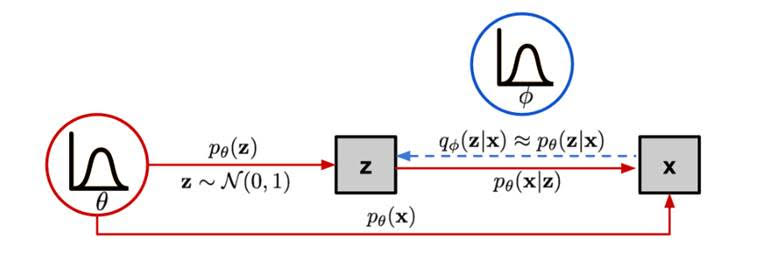
\includegraphics[width=0.75\linewidth]{media/arq_VAN.jpg}
\caption{Arquitectura general de un Autoencoder Variacional.}
\textbf{Fuente:} adaptado de \citeA{Weng2018}.
\label{fig:arq-vae}
\end{figure}

Por otro lado, las redes generativas adversarias, conocidas como GAN, son modelos generativos formados por dos redes neuronales que compiten entre sí mediante un proceso de entrenamiento adversarial: un generador y un discriminador. El generador trata de crear muestras sintéticas similares a los datos reales, mientras que el discriminador intenta distinguir entre las muestras reales y las generadas. A través de este proceso, el generador mejora progresivamente su capacidad para producir datos plausibles siguiendo la distribución de probabilidad de los datos utilizados durante el entrenamiento \cite{Goodfellow2014}.

Como puede observarse en la Figura~\ref{fig:arq-gan}, el proceso de entrenamiento de una GAN parte de un vector de ruido latente que es transformado por el generador en una muestra sintética. Posteriormente, el discriminador recibe tanto datos reales como datos generados y aprende a clasificarlos, proporcionando una señal que permite mejorar al generador durante el entrenamiento \cite{DeLaTorre2023}.

\begin{figure}[H]
\centering
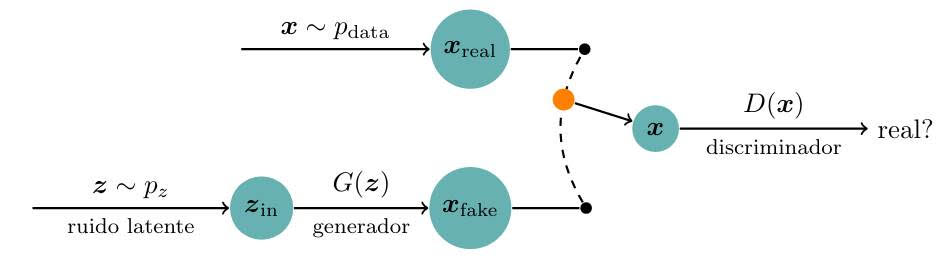
\includegraphics[width=0.75\linewidth]{media/proceso_GANs.jpg}
\caption{Diagrama representativo del proceso de entrenamiento de las redes generativas adversarias (GAN).}
\textbf{Fuente:} adaptado de \citeA{DeLaTorre2023}.
\label{fig:arq-gan}
\end{figure}

En el caso de datos financieros temporales, una GAN básica no resulta suficiente para representar de forma explícita la estructura secuencial de las observaciones. Por ese motivo, el modelo adversarial considerado en el experimento es TimeGAN, que adapta el aprendizaje generativo adversarial al tratamiento de series temporales mediante componentes de representación, recuperación y supervisión temporal.

Una vez presentados los conceptos fundamentales de la inteligencia artificial y los modelos generativos, se introduce el otro pilar del trabajo: la optimización de carteras y la teoría moderna de carteras. Este ámbito resulta esencial para entender cómo los escenarios sintéticos generados pueden trasladarse posteriormente a un problema de asignación de activos. 

Según \cite{Zhao2025}, la modernización por parte del consumidor y la creciente demanda de inversión han puesto la gestión de carteras en primer plano, siendo una base fundamental para la optimización de las mismas.

Dentro de este ámbito, el enfoque propuesto por \cite{Markowitz1952}, conocido como teoría moderna de carteras, constituye uno de los pilares fundamentales ya que plantea que una cartera no debe valorarse únicamente por la rentabilidad que puede generar, sino también por el riesgo que implica asumir dicha inversión.

En este artículo se define la teoría moderna de carteras como un enfoque financiero que permite construir carteras eficientes teniendo en cuenta la relación entre rentabilidad esperada y riesgo. Esta idea se encuentra directamente vinculada con el concepto de optimización de carteras, ya que optimizar una cartera implica seleccionar y asignar pesos a diferentes activos con el objetivo de alcanzar el mejor equilibrio posible entre el rendimiento esperado y el nivel de riesgo asumido.

De la idea de \cite{Markowitz1952} nace otro concepto muy importante relacionado con la optimización, la frontera eficiente. Esta representa las carteras que ofrecen mayor rentabilidad para un nivel de riesgo dado, de forma que una cartera situada sobre la frontera eficiente se considera óptima porque no existe otra combinación de activos que proporcione una mayor rentabilidad esperada para el mismo nivel de riesgo.

\begin{figure}[H]
\centering
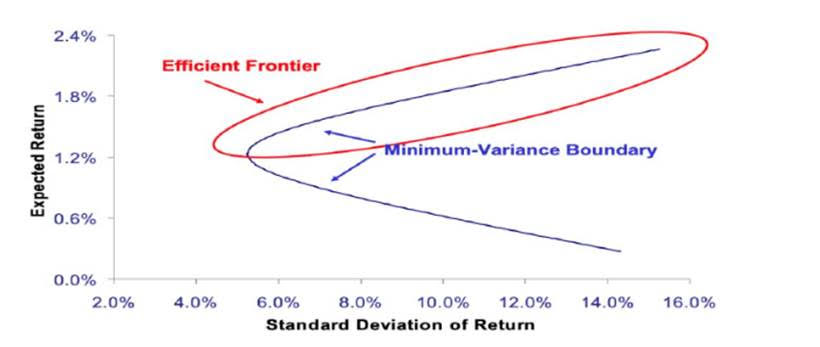
\includegraphics[width=0.75\linewidth]{media/FronteraEficiente.jpg}
\caption{Representación de la frontera eficiente y la frontera de mínima varianza.}
\textbf{Fuente:} tomado de \citeA[p.~1563, Fig.~1]{Hu2022}.
\label{fig:frontera-eficiente-minima-varianza}
\end{figure}

Con el fin de medir la distancia entre las distribuciones de retorno reales y las generadas se recurrirá a técnicas basadas en la teoría de la información, la cual ha quedado correctamente definida por \cite{Shannon1948} como una teoría matemática representada mediante un esquema general de comunicación que permite cuantificar la información generada por una fuente a partir de la incertidumbre asociada a sus posibles mensajes.

\begin{figure}[H]
\centering
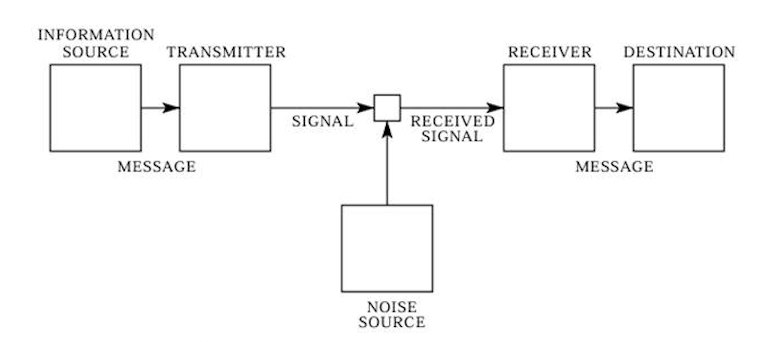
\includegraphics[width=0.75\linewidth]{media/esquema_sistComunicacion.png}
\caption{Esquema general de un sistema de comunicación.}
\textbf{Fuente:} tomado de \citeA[Fig.~1]{Shannon1948}.
\label{fig:sistema-comunicacion-shannon}
\end{figure}

Aunque el esquema original de Shannon se plantea dentro del contexto de los sistemas de comunicación, su principal aportación consiste en formalizar la información como una magnitud cuantificable. Esta idea puede trasladarse al contexto del análisis de datos y del aprendizaje automático. En este sentido, como señalan \citeA{AlvarezChaves2024}, la entropía, la información mutua y la divergencia de Kullback--Leibler (KL) son conceptos fundamentales de la teoría de la información.

En él se define la entropía de una variable aleatoria X como el contenido medio de información de cada uno de sus posibles resultados, cuantificando así el grado de incertidumbre o variabilidad asociado a dicha variable, y siendo la misma una medida a utilizar en nuestro futuro desarrollo. 

Como puede observarse en la Figura~\ref{fig:entropia-shannon}, la entropía alcanza su valor máximo cuando la incertidumbre es mayor, es decir, cuando todos los resultados posibles son equiprobables y ninguno de ellos aporta más información que otro.

\begin{figure}[H]
\centering
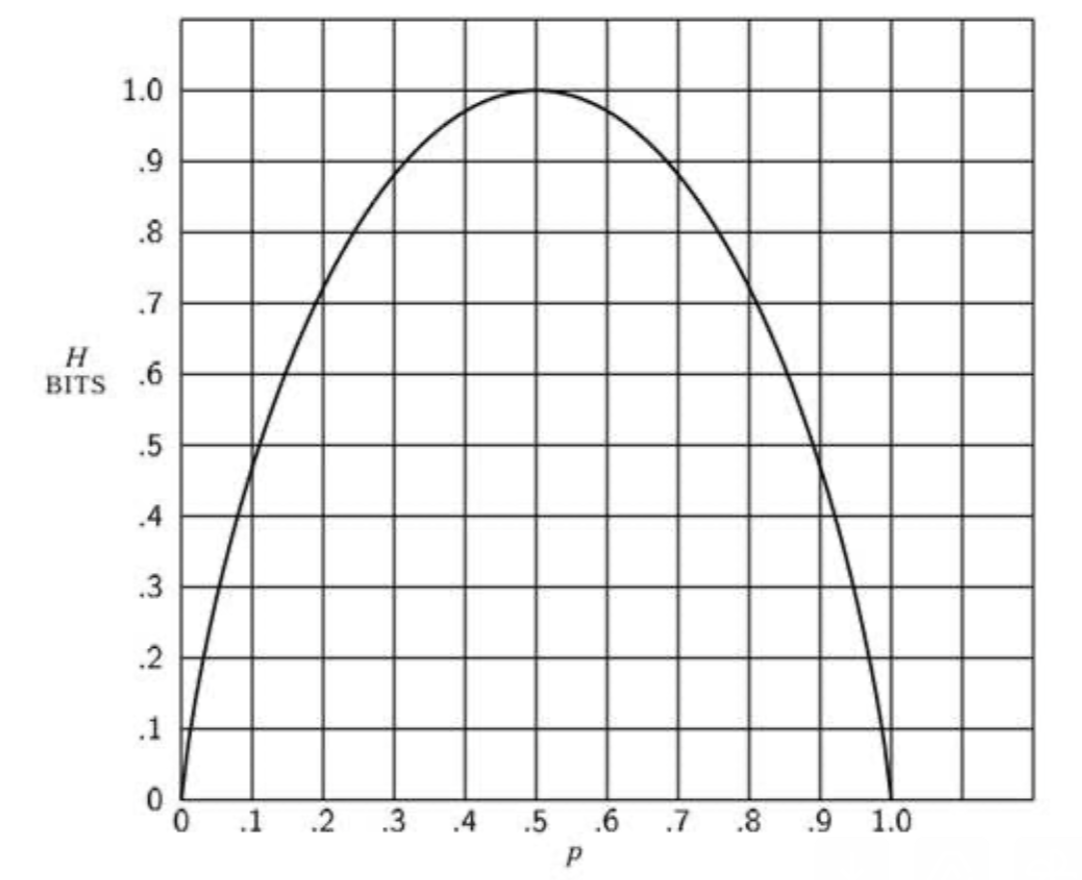
\includegraphics[width=0.7\linewidth]{media/entropia.png}
\caption{Entropía en el caso de dos posibles resultados con probabilidades $p$ y $(1-p)$.}
\textbf{Fuente:} tomado de \citeA[Fig.~7]{Shannon1948}.
\label{fig:entropia-shannon}
\end{figure}

También establece la divergencia de Kullback-Leibler que permite medir la diferencia entre dos distribuciones de probabilidad definidas sobre el mismo espacio, puede interpretarse como la ineficiencia que se produce al asumir que la distribución es Q cuando la distribución verdadera es P. Esta métrica resulta especialmente útil para comparar la distribución de retornos reales con la distribución generada por el modelo, permitiendo evaluar hasta qué punto los escenarios sintéticos reproducen el comportamiento estadístico de los datos originales.

La Figura\ref{fig:kullback-leibler} muestra visualmente dos distribuciones y cómo la divergencia KL permite comparar la diferencia entre ellas, de forma que, una menor divergencia entre la distribución real y la generada indicaría que el modelo reproduce de forma más precisa el comportamiento estadístico de los retornos financieros.

\begin{figure}[H]
\centering
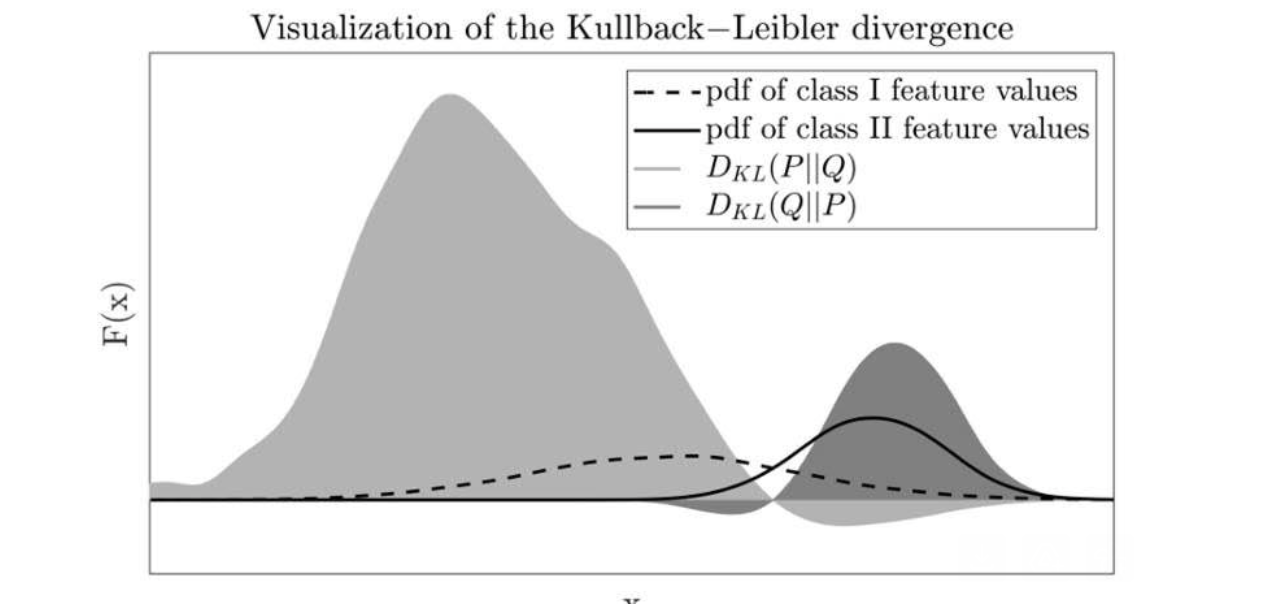
\includegraphics[width=0.8\linewidth]{media/Kullback-Leibler.png}
\caption{Representación visual de la divergencia de Kullback-Leibler entre dos distribuciones de probabilidad.}
\textbf{Fuente:} tomado de \citeA[Fig.~4]{Lysiak2021}.
\label{fig:kullback-leibler}
\end{figure}

Por último, \cite{AlvarezChaves2024} define la información mutua como una métrica que permite medir la dependencia existente entre dos variables aleatorias, cuantificando la reducción media de incertidumbre sobre una variable X cuando se conoce otra variable Y. Esto la convierte en una herramienta esencial para el presente trabajo, ya que permite estudiar si el modelo es capaz de guardar las relaciones existentes entre los activos financieros incluyendo aquellas dependencias que otros enfoques podrían pasar por alto.

En este contexto, la combinación de modelado generativo y teoría de la información se presenta como una línea de investigación prometedora para abordar el problema de la optimización de carteras desde una perspectiva más flexible y realista. Este enfoque permite no solo generar escenarios plausibles del mercado, sino también evaluar su calidad y utilidad en la toma de decisiones, lo que constituye la base sobre la que se desarrolla el presente trabajo.

\section{Estado del arte}
\subsection{Antecedentes}
La optimización de carteras ha evolucionado desde modelos clásicos basados en la relación entre riesgo y rentabilidad hasta enfoques avanzados apoyados en aprendizaje automático y teoría de la información. El punto de partida fue la teoría moderna de carteras de Markowitz \cite{Markowitz1952}, que introdujo el concepto de frontera eficiente y el principio de diversificación, según el cual la combinación de activos permite reducir el riesgo total de la cartera.


\begin{figure}[H]
\centering
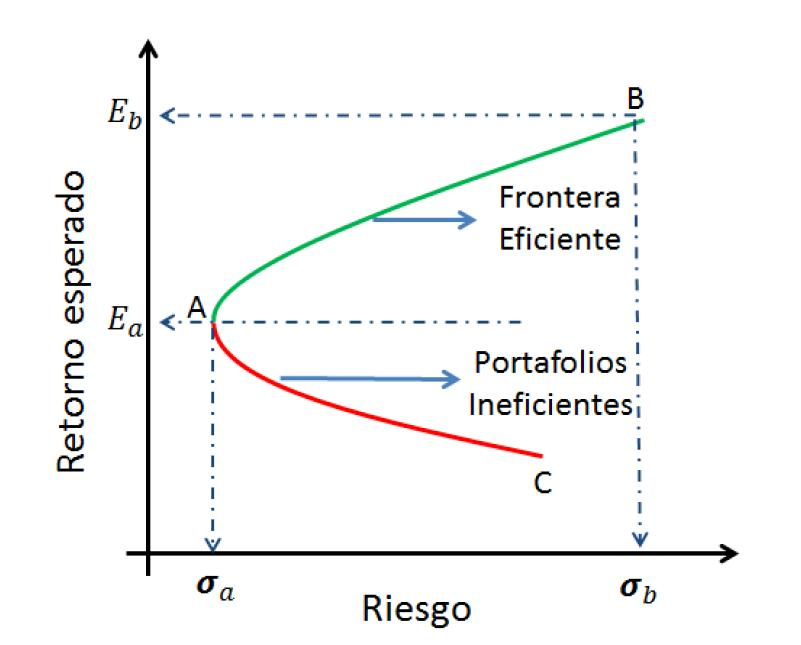
\includegraphics[width=0.7\linewidth]{media/relacion riesgo-rentabilidad.jpg}
\caption{Representación de la frontera eficiente en el marco de la teoría moderna de carteras.}
\textbf{Fuente:} tomado de Gómez y Jiménez (2020), basado en Markowitz (1952).
\label{fig:frontera_eficiente}
\end{figure}

Como se observa en la Figura~\ref{fig:frontera_eficiente}, la frontera eficiente representa las carteras que ofrecen la mayor rentabilidad esperada para cada nivel de riesgo, mientras que las combinaciones situadas por debajo de ella se consideran ineficientes.

La diversificación constituye uno de los principales aportes de este enfoque, ya que permite disminuir el riesgo específico de la cartera mediante la incorporación de activos con comportamientos diferentes.

\begin{figure}[H]
\centering
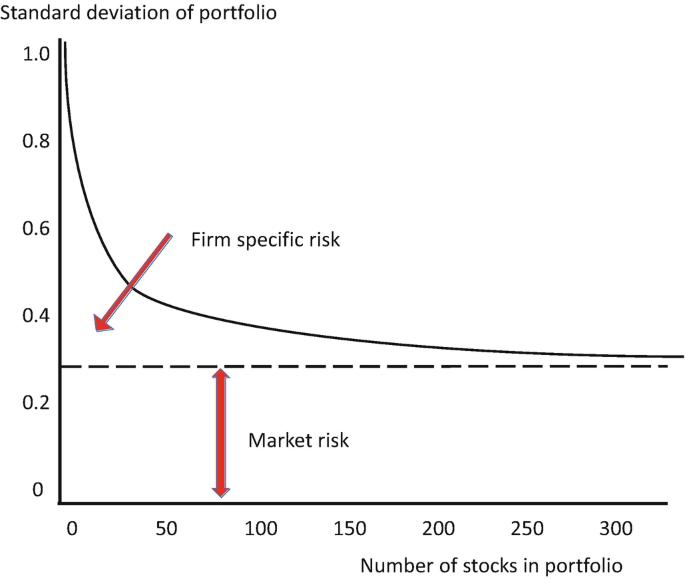
\includegraphics[width=0.7\linewidth]{media/diversificación en la reducción del riesgo.jpg}
\caption{Efecto de la diversificación en la reducción del riesgo de una cartera.}
\textbf{Fuente:} tomado de Schoenmaker y Schramade (2023), adaptado de Statman (2004).
\label{fig:diversificacion}
\end{figure}

La Figura~\ref{fig:diversificacion} muestra que el riesgo total disminuye conforme aumenta el número de activos en la cartera. Sin embargo, esta reducción tiene un límite asociado al riesgo sistemático o de mercado, que no puede eliminarse mediante diversificación.

Posteriormente surgieron modelos como el CAPM de Sharpe \cite{Sharpe1964}, que relaciona la rentabilidad esperada de un activo con su riesgo sistemático. Más adelante, los modelos ARCH y GARCH \cite{Bollerslev1986} permitieron representar la volatilidad variable en el tiempo, mientras que el modelo Black-Litterman \cite{BlackLitterman1992} incorporó información del mercado y expectativas del inversor para obtener carteras más estables.

En paralelo, el aumento en la disponibilidad de datos financieros y el desarrollo de nuevas capacidades computacionales favorecieron la incorporación de técnicas de aprendizaje automático en el análisis financiero. En el ámbito de la optimización de carteras, esto ha dado lugar a propuestas como la Deep Portfolio Theory, que utiliza redes neuronales profundas para aprender representaciones latentes de los activos y construir carteras a partir de dichas representaciones \cite{Heaton2016}.

Más recientemente, los modelos generativos han adquirido una relevancia creciente y han comenzado a aplicarse en finanzas. A diferencia de los modelos predictivos tradicionales, que se centran en estimar valores esperados, los modelos generativos buscan aprender la distribución de los datos para generar nuevas muestras coherentes con el comportamiento observado. Entre estos modelos destacan los autoencoders variacionales (VAE), que permiten aprender representaciones probabilísticas en espacios latentes \cite{Kingma2013}, y TimeGAN, que adapta el aprendizaje adversarial a la generación de series temporales mediante componentes de embedding, recuperación y supervisión temporal \cite{Yoon2019}.

\begin{figure}[htbp]
    \centering
    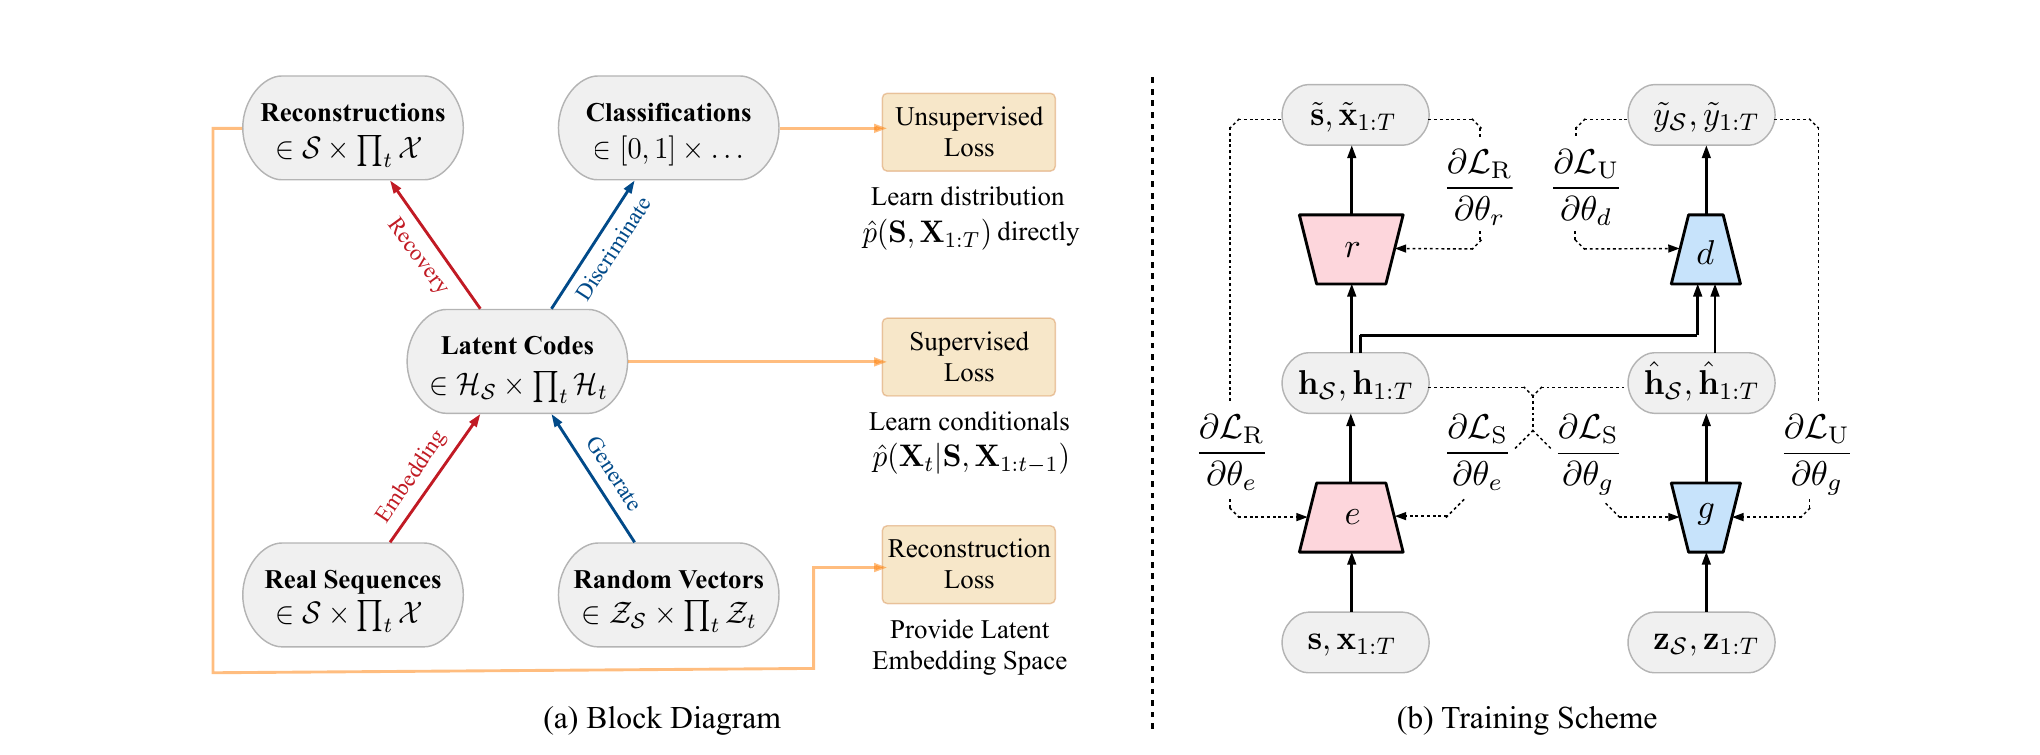
\includegraphics[width=\textwidth]{media/timegan_yoon2019_fig1.png}
    \caption{Esquema conceptual de TimeGAN como modelo generativo temporal: diagrama de bloques funcionales y esquema de entrenamiento.}
    \textbf{Fuente:} tomado de la Figura 1 de Yoon et al. \cite{Yoon2019}.
    \label{fig:timegan-externo}
\end{figure}


En el contexto financiero, estos modelos ofrecen la posibilidad de generar escenarios sintéticos del comportamiento del mercado. En esta línea, trabajos como el de Mariani, \cite{Mariani2019} han explorado el uso de modelos generativos en el análisis de carteras, mostrando su potencial como herramienta complementaria para estudiar la incertidumbre y el riesgo.

Paralelamente, la teoría de la información ha comenzado a desempeñar un papel relevante en el análisis financiero, al proporcionar herramientas para cuantificar la incertidumbre y medir la diferencia entre distribuciones probabilísticas. Conceptos como la entropía, la divergencia de Kullback-Leibler o la información mutua permiten analizar las propiedades de las distribuciones de los retornos desde una perspectiva más general que la ofrecida por las medidas tradicionales \cite{Kullback1951}. En particular, estas métricas permiten capturar dependencias no lineales entre variables y evaluar la calidad de modelos probabilísticos, lo que resulta especialmente útil en el contexto de los modelos generativos.

En los últimos años, diversos trabajos han explorado la integración de estas métricas en el proceso de optimización de carteras, proponiendo enfoques que combinan rentabilidad, riesgo e información. En este sentido, el uso de medidas como la entropía o la información mutua permite estudiar relaciones más complejas entre activos \cite{Novais2022}. Este tipo de propuestas refleja una tendencia hacia modelos capaces de representar tanto la incertidumbre como la estructura de dependencia entre variables.

En conjunto, los antecedentes analizados muestran una evolución progresiva en la forma de abordar la optimización de carteras. Desde los modelos clásicos basados en supuestos simplificados hasta los enfoques más recientes fundamentados en aprendizaje automático y teoría de la información, se observa una tendencia clara hacia metodologías más flexibles, capaces de capturar la complejidad del mercado financiero. Esta evolución pone de manifiesto la necesidad de integrar distintas herramientas y enfoques para desarrollar modelos más realistas y robustos, lo que constituye la base sobre la que se plantea el presente trabajo. 

Esta evolución puede resumirse de forma esquemática en la siguiente representación.

\begin{figure}[H]
\centering
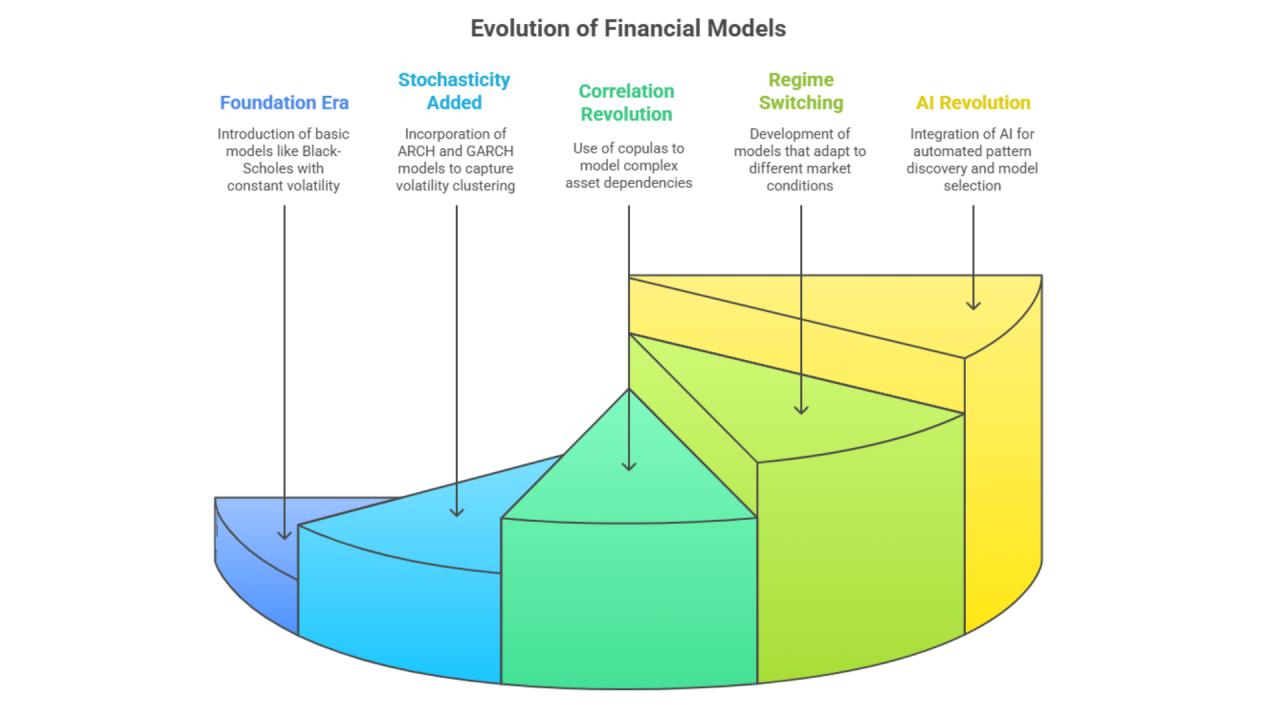
\includegraphics[width=0.7\linewidth]{media/evolucion-modelos.jpg}
\caption{Evolución de los enfoques de optimización de carteras desde modelos clásicos hasta técnicas avanzadas.}
\textbf{Fuente:} tomado de Kheria (2025).
\label{fig:evolucion}
\end{figure}

Como se muestra en la Figura~\ref{fig:evolucion}, la optimización de carteras ha evolucionado desde modelos clásicos basados en supuestos simplificados hacia metodologías más flexibles basadas en datos, inteligencia artificial y aprendizaje automático, capaces de capturar mejor la complejidad de los mercados financieros.

\subsection{Limitaciones de los enfoques tradicionales}

A pesar de su importancia en el desarrollo de la teoría financiera moderna, los enfoques tradicionales de optimización de carteras presentan diversas limitaciones que dificultan su aplicación en entornos financieros reales. En particular, el modelo media-varianza de Markowitz depende de estimaciones precisas de medias, varianzas y covarianzas obtenidas a partir de datos históricos. Esto provoca una elevada sensibilidad a errores de estimación, generando carteras inestables y poco robustas \cite{Markowitz1952,BlackLitterman1992}.

Además, estos modelos suelen asumir que los mercados son relativamente estables y que los retornos siguen distribuciones normales. Sin embargo, la evidencia empírica muestra que los retornos financieros presentan colas pesadas, asimetrías y episodios de volatilidad agrupada, fenómenos que los enfoques clásicos no logran representar adecuadamente \cite{Bollerslev1986}. Como consecuencia, el riesgo de eventos extremos puede ser subestimado.

Otra limitación importante es el uso de la varianza como medida principal de riesgo, ya que esta no distingue entre desviaciones positivas y negativas. Asimismo, las medidas tradicionales de dependencia, como la correlación, solo capturan relaciones lineales entre activos y no reflejan adecuadamente las dependencias complejas que suelen aparecer en periodos de estrés financiero.

La diferencia entre el supuesto teórico de normalidad y el comportamiento real de los retornos financieros puede observarse en la siguiente figura.

\begin{figure}[H]
\centering
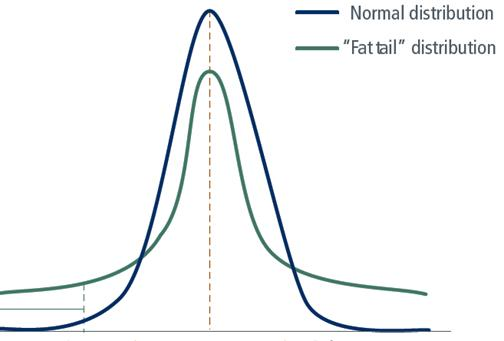
\includegraphics[width=0.65\linewidth]{media/distribucion normal-distribucion cola.jpg}
\caption{Comparación entre una distribución normal y una distribución de retornos financieros con colas pesadas.}
\textbf{Fuente:} tomado de SAS (2015).
\label{fig:distribucion}
\end{figure}

Como se aprecia en la Figura~\ref{fig:distribucion}, los retornos financieros presentan una mayor probabilidad de eventos extremos en comparación con la distribución normal, lo que evidencia una de las principales limitaciones de los modelos tradicionales.

En conjunto, estas limitaciones han impulsado el desarrollo de enfoques más flexibles, capaces de modelar distribuciones completas, capturar dependencias no lineales y representar de forma explícita la incertidumbre en los mercados financieros.

\subsection{Teoría de la información aplicada a la optimización de carteras}

La teoría de la información proporciona herramientas matemáticas para analizar la incertidumbre y las dependencias entre variables aleatorias, ofreciendo una perspectiva más flexible que los enfoques tradicionales basados únicamente en la varianza y la correlación.

En este contexto, la entropía permite medir el grado de incertidumbre o dispersión de los retornos financieros sin asumir distribuciones normales. Por su parte, la divergencia de Kullback-Leibler permite cuantificar la diferencia entre distribuciones probabilísticas \cite{Kullback1951}, siendo especialmente útil para evaluar modelos generativos capaces de reproducir el comportamiento del mercado.

Asimismo, la información mutua permite capturar dependencias no lineales entre activos financieros, superando algunas limitaciones de la correlación lineal tradicional. En este sentido, distintos enfoques recientes han propuesto incorporar métricas como la entropía o la información mutua al análisis de carteras, con el objetivo de estudiar la diversificación desde una perspectiva informacional \cite{Novais2022}.

La relación entre la teoría de la información y los modelos generativos refuerza su relevancia en este contexto. Muchos modelos generativos modernos, como los autoencoders variacionales, incorporan explícitamente la divergencia de Kullback-Leibler en su función de optimización, lo que conecta el aprendizaje de distribuciones con las métricas informacionales. Esta integración permite no solo generar escenarios probabilísticos, sino también evaluar su calidad dentro de un marco de validación más amplio.

En consecuencia, la teoría de la información puede complementar la medición tradicional del riesgo y de la dependencia entre activos, además de facilitar la evaluación de modelos generativos. Esta combinación resulta relevante para estudiar enfoques capaces de representar la incertidumbre y la dinámica del mercado financiero desde una perspectiva más distribucional.

De forma esquemática, el funcionamiento general de este tipo de modelos puede entenderse como un proceso de aprendizaje de la distribución de los datos para posteriormente generar nuevas muestras sintéticas coherentes con ella.

\begin{figure}[htbp]
\centering
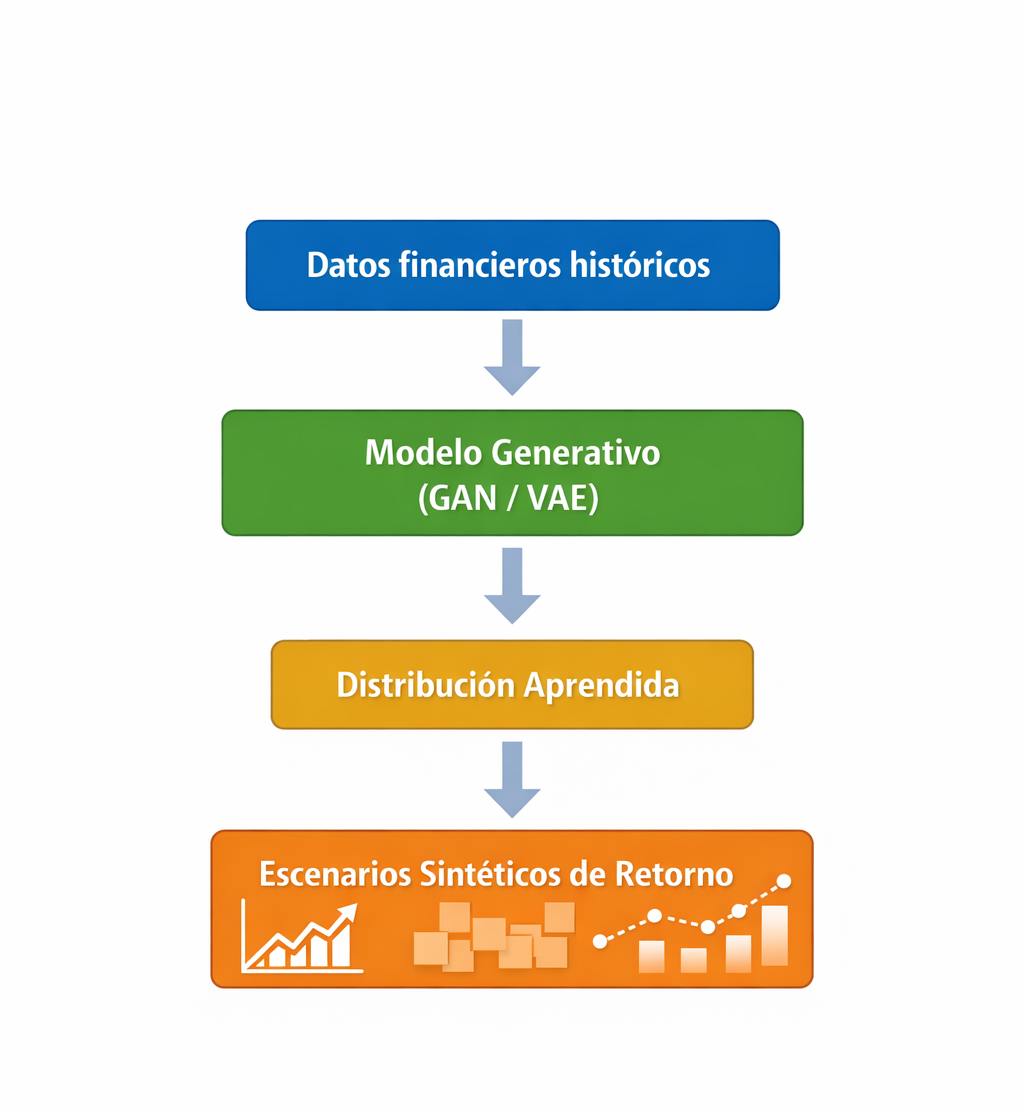
\includegraphics[width=0.55\linewidth]{media/Modelo generativo.png}
\caption{Esquema conceptual del enfoque propuesto, integrando modelos generativos y métricas de teoría de la información para la optimización de carteras.}
\textbf{Fuente:} elaboración propia.
\label{fig:modelo}
\end{figure}

Como muestra la Figura~\ref{fig:modelo}, estos modelos permiten aprender una representación de los datos financieros históricos para posteriormente generar escenarios sintéticos coherentes con el comportamiento observado. En este trabajo, dichos escenarios se analizan como una herramienta complementaria para estudiar el riesgo y apoyar el proceso de optimización de carteras.

\subsection{Estudios actuales}

En los últimos años, la investigación en optimización de carteras ha experimentado una gran evolución, impulsada tanto por los avances en la inteligencia artificial como por una comprensión más profunda de los mercados financieros. Esto ha permitido que actualmente sean muchos los sistemas capaces de representar de forma adecuada la complejidad de los mercados financieros, evolucionando progresivamente desde representaciones simples del retorno esperado hasta modelos más complejos que permiten modelar la incertidumbre del mercado y las dependencias existentes entre los activos. Esta evolución representa la necesidad de desarrollar herramientas que se ajusten de forma realista al comportamiento observado en los mercados, lo que lleva a proponer un enfoque diferenciado basado en dos componentes fundamentales que actúan de forma complementaria: el empleo de modelos generativos para caracterizar el comportamiento del mercado y la incorporación de métricas procedentes de la teoría de la información para evaluar la calidad del modelo.


Para situar nuestro proyecto dentro de la situación académica actual e identificar su aportación diferencial respecto a investigaciones ya realizadas, se presentan a continuación algunos de los estudios más recientes, los cuales se orientan hacia el desarrollo de modelos capaces de generar distribuciones y predicciones probabilísticas útiles para la toma de decisiones, sirviendo como base para la contextualización de la propuesta desarrollada en este trabajo.


Uno de los trabajos más relevantes en este contexto es el realizado por \cite{Huang2024}, en el que los autores proponen un enfoque dividido en dos etapas para construir y optimizar carteras de inversión. En vez de centrarse únicamente en cómo repartir los pesos de los activos, los autores separan el proceso en una primera fase de selección de activos, en la que desarrollan un modelo que combina técnicas actuales como redes convolucionales, grafos y relaciones de vecindad entre activos y una segunda de optimización del modelo desarrollado.

La utilidad de este estudio para el presente trabajo reside en la tendencia que refleja: construir u optimizar una cartera no siempre puede tratarse como un problema estático de una sola etapa, sino como un proceso en el que intervienen varias decisiones encadenadas. Aunque en este estudio no se emplean modelos generativos, su planteamiento ayuda a contextualizar la necesidad de modelos con mayor capacidad para captar patrones complejos en datos financieros, especialmente cuando las relaciones entre activos no son lineales y no pueden resumirse únicamente mediante media, varianza y covarianza. Esta idea se relaciona con el objetivo de este proyecto, aunque aquí se adopta un enfoque distinto basado en modelos generativos y métricas informacionales para evaluar escenarios probabilísticos de retornos.

Otro de los estudios relevantes, relacionado con esta línea de investigación, es el realizado por \cite{Kalina2024}, en el que se emplean modelos variacionales encoder-decoder para desarrollar un método de aumento de datos financieros. El punto de partida de esta investigación son dos problemas frecuentes en el ámbito financiero: la escasez de datos para entrenar modelos complejos y la pérdida de diversidad de escenarios cuando solo se cuenta con una trayectoria observada. Para abordar este problema, los autores proponen descomponer las series financieras en componentes como tendencia y dispersión, y modelar nuevas estructuras de datos más representativas. Los resultados indican que incorporar estos escenarios generados puede producir mejoras apreciables en el rendimiento de las carteras dentro del marco experimental analizado por los autores.

Este trabajo resulta muy útil para el presente proyecto por varias razones. En primer lugar, pone en manifiesto la escasez de datos destinados a investigación en este tipo de contexto, lo que limita al desarrollo de modelos para generalizar correctamente y capturar la complejidad de los mercados financieros. En segundo lugar, demuestra que los modelos variacionales no se limitan exclusivamente a reducir dimensionalidad, sino que también son capaces de reconstruir y generar series financieras con propiedades coherentes. En tercer lugar, introduce que la calidad de un modelo generativo no debería medirse sólo en términos de similitud visual con los datos reales, también debemos tener en cuenta la capacidad del mismo para preservar patrones del mercado y mejorar tareas concretas como la construcción de carteras o la toma de decisiones. Por último, compara varias técnicas de inteligencia artificial, como el aprendizaje federado (FED) o redes generativas de series temporales (TimeGan), esto demuestra que la búsqueda de la mejor aproximación para la optimización de carteras sigue siendo una cuestión sin resolver, lo que deja margen para propuestas como la de este trabajo.

Aunque los resultados del estudio muestran mejoras en el rendimiento de cartera bajo su protocolo experimental, su objetivo no coincide plenamente con el de este TFM. En este trabajo, el interés se centra específicamente en evaluar VAE y TimeGAN como generadores de escenarios y en contrastar dichos escenarios mediante métricas estadísticas, temporales e informacionales antes de su uso en optimización.


Para acabar con los estudios realizados durante el 2024, y antes de empezar con algunas contribuciones más recientes, resulta relevante destacar la línea de investigación centrada en modelos de difusión aplicados a series financieras. En este contexto, uno de los trabajos más influyentes es FTS-Diffusion, presentado en ICLR 2024 \cite{FTSDiffusion2024}.


En este trabajo, los autores parten de la idea de que las series financieras presentan dos dificultades relevantes para su modelado: la irregularidad y la presencia de patrones a distintas escalas temporales. Para abordar este problema proponen una arquitectura generativa formada por tres módulos: reconocimiento de patrones, generación mediante difusión y evaluación temporal. Los resultados obtenidos indican que el modelo es capaz de generar datos artificiales con propiedades próximas a las observadas en el mercado real y que, al utilizar estos datos en tareas posteriores, se reduce el error de predicción en torno a un 17,9\% en los experimentos descritos por los autores.


Este estudio resulta relevante para nuestro proyecto ya que emplea modelos de difusión, que actualmente pueden suponer un avance respecto a modelos clásicos al aportar una mayor estabilidad en el entrenamiento y una mejor capacidad para generar muestras de mayor calidad. Sin embargo, este enfoque se centra sobre todo en la generación de datos y su aplicación en tareas concretas, sin incluir métricas basadas en teoría de la información que permitan evaluar la calidad de los resultados obtenidos, por lo que nuestro proyecto introduce una aportación diferente: combinar el uso de modelos generativos con medidas basadas en teoría de la información, lo que permite no solo generar escenarios posibles del mercado, sino también medir de forma explícita la distancia entre las distribuciones reales y las generadas antes de utilizarlas para la optimización de carteras.


En una línea diferente y volviendo un poco hacía atrás en el tiempo, \cite{Novais2022} ha propuesto un modelo de optimización de cartera que integra la media, la entropía y la información mutua. Este modelo busca representar de forma más completa la incertidumbre y las dependencias entre los activos financieros mediante el uso de métricas informacionales en lugar de la varianza y la covarianza tradicionales, de forma que permitan capturar relaciones más complejas entre los activos. Los resultados indican que estos modelos no siempre logran superar en rentabilidad a enfoques como el de media-varianza o a algunas técnicas robustas, pero sí muestran ventajas en cuanto a estabilidad y diversidad en la asignación de pesos, aspecto importante en este tipo de contextos.


Este trabajo resulta especialmente útil porque aborda una forma alternativa de medir la incertidumbre y las relaciones entre activos que no depende únicamente de las correlaciones lineales clásicas. La propuesta muestra que métricas como la entropía o la información mutua pueden desempeñar un papel relevante en la construcción y optimización de carteras, mientras que otros enfoques se centran principalmente en reproducir trayectorias o mejorar la capacidad predictiva de los modelos. Además, el estudio refuerza una de las ideas sobre las que se apoya este trabajo: las medidas de teoría de la información no son solo herramientas matemáticas para comparar distribuciones, sino que también pueden tener una interpretación financiera concreta.

Entre las contribuciones más recientes, destaca el trabajo de \cite{Gao2025}, en el que se propone un modelo basado en transformers diseñado para optimizar carteras en función del contexto del mercado. El punto de partida de esta investigación es una crítica a los métodos convencionales apoyados en estimaciones puntuales de retornos, ya que pueden representar de forma limitada la incertidumbre y las dependencias entre activos. Como alternativa, los autores proponen un modelo que aprende la distribución condicional de los retornos futuros a partir de factores observables de cada activo en el tiempo. Estas distribuciones se integran posteriormente mediante estrategias basadas en media y varianza. Los resultados descritos por los autores sugieren que una caracterización probabilística más completa de los retornos puede mejorar el comportamiento de las carteras bajo su protocolo experimental.

Este estudio resulta relevante para este trabajo ya que se aproxima de manera directa a nuestro objetivo principal: emplear modelos generativos como mecanismo para aprender distribuciones de retorno que posteriormente se puedan integrar de forma explícita en el proceso de optimización de carteras. No obstante, el planteamiento dado se orienta exclusivamente a la generación de distribuciones condicionales y a su aplicación directa en la optimización, sin contemplar una forma que permita valorar de manera precisa la calidad de las distribuciones más allá de los resultados obtenidos.


Frente a este último aspecto, nuestro proyecto continúa planteando una aportación diferenciada al combinar el uso de modelos generativos con métricas procedentes de teoría de la información, que permitirán cuantificar con precisión cuánto se alejan las distribuciones generadas de las reales. De este modo, el objetivo no se limita a mejorar la representación probabilística de los retornos, sino también a contar con un criterio formal que permita verificar la fidelidad del modelo antes de trasladar sus resultados a la toma de decisiones.

Para cerrar los estudios más recientes, cabe destacar el enfoque de modelado distribucional presentado por \cite{Diffolio2026}, en el que se desarrolla un modelo de difusión multivariante orientado tanto a la predicción probabilística de series financieras como a la construcción de carteras. Según el resumen del artículo, el modelo combina una red de desruido con un sistema de atención que analiza tanto cada activo como el mercado en general, incluyendo un mecanismo basado en correlaciones para reflejar relaciones entre activos. Los experimentos descritos por los autores indican mejoras frente a varios modelos de referencia en las tareas evaluadas, aunque sus resultados deben interpretarse dentro del protocolo concreto del estudio.

Desde el punto de vista del presente trabajo, esta investigación pone de manifiesto que las tendencias actuales están centradas en el desarrollo de modelos capaces de aprender distribuciones conjuntas sobre múltiples activos, teniendo en cuenta las relaciones existentes entre ellos. Este aspecto resulta fundamental, ya que nos recuerda que el comportamiento de una cartera no puede entenderse únicamente a partir de cada activo de forma independiente, sino que depende en gran medida de cómo estos interactúan entre sí. En consecuencia, los enfoques que se desarrollen en este proyecto han de ser capaces no solo de generar retornos individuales, sino de preservar también las dependencias cruzadas que caracterizan a los mercados financieros reales. 



Si se observan en conjunto los estudios analizados, se aprecia una evolución en la forma de plantear la optimización de carteras. Frente a modelos formulados como un único problema estático, trabajos recientes como el de \citeA{Huang2024} proponen procesos de decisión más encadenados. Por otro lado, la propuesta de \citeA{Kalina2024} abre otra vía de interés, en la que la generación de datos sintéticos puede actuar como herramienta auxiliar para estudiar carteras bajo escenarios más variados.

En muchos de los estudios se observa un interés creciente por los modelos generativos y por la representación distribucional de los retornos. Propuestas como FTS-Diffusion, \citeA{Gao2025} o Diffolio plantean la importancia de aprender distribuciones financieras en lugar de limitarse a estimar un valor esperado puntual. Este cambio permite analizar de forma más explícita la incertidumbre y las relaciones entre activos. También se detecta una preocupación creciente por evaluar estos modelos no solo en términos de similitud con los datos reales, sino por su efecto cuando se aplican a tareas concretas como la predicción o la construcción de carteras. Este último aspecto conecta directamente con uno de los objetivos centrales del presente proyecto.

Por último, muchas de las investigaciones revisadas cuestionan que las correlaciones lineales sean suficientes para comprender cómo se relacionan los activos entre sí, y proponen sustituirlas o complementarlas con otras medidas como la entropía o la información mutua. La conclusión relevante para este trabajo es que existen métricas capaces de describir dependencias que los métodos tradicionales pueden no recoger adecuadamente. Por ello, resulta importante no solo generar escenarios, sino también medir de forma rigurosa su calidad.

En conclusión, a partir de los estudios analizados se observa que la optimización de carteras constituye un ámbito de investigación ampliamente desarrollado, con numerosas propuestas orientadas a mejorar la modelización del mercado y el análisis de decisiones de inversión. En este contexto, el presente trabajo se sitúa como una contribución acotada: integra modelado generativo y métricas de teoría de la información en un flujo experimental reproducible para estudiar la generación de escenarios probabilísticos y su posible uso en la optimización de carteras.

A continuación se presenta una tabla resumen con los estudios mencionados, destacando su principal aportación y las limitaciones encontradas respecto al presente proyecto.

{\small
\renewcommand{\arraystretch}{1.2}
\begin{longtable}{|p{2.5cm}|p{5.5cm}|p{5.5cm}|}
\caption{Resumen de los estudios actuales y su limitación respecto al presente proyecto}\label{tab:estudios_actuales} \\
\hline
\textbf{Estudio} & \textbf{Aportación principal} & \textbf{Limitación encontrada} \\
\hline
\endfirsthead

\hline
\textbf{Estudio} & \textbf{Aportación principal} & \textbf{Limitación encontrada} \\
\hline
\endhead

\hline
\multicolumn{3}{r}{\textit{Continúa en la siguiente página}} \\
\endfoot

\hline
\endlastfoot

Huang et al. (2024) &
Propone un enfoque en dos etapas para la construcción y optimización de carteras, separando la selección de activos de la optimización final. &
No emplea modelos generativos ni métricas de teoría de la información. \\
\hline

Kalina et al. (2024) &
Genera datos financieros sintéticos a través de modelos variacionales produciendo resultados  más sólidos que no dependen de un único escenario de mercado. &
No evalúa la calidad de las distribuciones con métricas de teoría de la información. \\
\hline

FTS-Diffusion (2024) &
Genera series financieras realistas mediante modelos de difusión. &
No incorpora evaluación con teoría de la información ni conexión directa con optimización. \\
\hline

Novais et al. (2022) &
Utiliza entropía e información mutua para modelar incertidumbre y dependencias entre activos. &
No combina estas métricas con modelos generativos. \\
\hline

Gao et al. (2025) &
Aprende distribuciones condicionales de retorno para optimización de carteras. &
No valida la calidad de las distribuciones generadas. \\
\hline

Diffolio (2026) &
Desarrolla un modelo de difusión multivariante que captura dependencias entre activos y mejora rendimiento de cartera. &
No integra métricas de teoría de la información para medir la distancia entre distribuciones reales y generadas. \\
\hline


\end{longtable}
}

\subsection{Herramientas existentes}

En la actualidad existen numerosas herramientas que permiten trabajar con datos financieros, entrenar modelos de aprendizaje automático y construir carteras de inversión. Sin embargo, la mayoría de ellas están pensadas para resolver solo una parte del problema. Por eso, cuando se quiere abordar una tarea más completa, como la que se plantea en este trabajo, normalmente es necesario combinar varias bibliotecas y frameworks dentro de un mismo flujo de trabajo.

En primer lugar, conviene distinguir entre herramientas generales y herramientas más específicas del ámbito financiero. Bibliotecas como \emph{pandas} y \emph{NumPy} no son herramientas financieras en sentido estricto, sino librerías de propósito general muy utilizadas en ciencia de datos, análisis numérico y aprendizaje automático. Aun así, resultan fundamentales en este tipo de trabajos porque facilitan tareas como la carga de series temporales, el cálculo de retornos, la alineación de fechas o el tratamiento de valores perdidos \cite{Harris2020,McKinney2010}.

Junto a estas librerías generales, existen herramientas más específicas para la obtención de datos de mercado, como \emph{yfinance}, que facilita el acceso a series históricas a través de \emph{Yahoo Finance}, o servicios externos como \emph{Alpha Vantage}. Estas soluciones resultan especialmente útiles en la fase inicial del trabajo, ya que permiten recopilar y preparar datos reales de activos financieros de forma relativamente sencilla. No obstante, su función se limita sobre todo a la obtención y preparación de datos, sin cubrir por sí mismas la parte de generación de escenarios ni la optimización de carteras.

Desde un punto de vista metodológico, este primer grupo de herramientas cumple una función crítica: garantizar que el conjunto de datos sobre el que se entrenarán los modelos sea consistente y comparable entre activos. En un problema de cartera, pequeñas diferencias en la alineación temporal de las series, en el tratamiento de días sin cotización o en la gestión de valores faltantes pueden alterar de forma apreciable las estimaciones posteriores. Por ello, el papel de estas librerías no debe entenderse solo como una ayuda técnica para manipular datos, sino como una base necesaria para asegurar la calidad de los análisis y la fiabilidad de los resultados.

En segundo lugar, para el desarrollo de modelos generativos destacan frameworks de aprendizaje profundo como \emph{TensorFlow} y \emph{PyTorch}, que tampoco son específicos de finanzas, sino herramientas generales de deep learning muy extendidas en múltiples áreas \cite{Abadi2016,Paszke2019}. Su interés en este proyecto radica en que ofrecen la flexibilidad necesaria para implementar arquitecturas como TimeGAN y los Autoencoders Variacionales (VAE), adaptando el entrenamiento a la estructura de los datos financieros. Aun así, requieren un diseño adicional para representar correctamente aspectos como la dependencia entre activos, la volatilidad o el comportamiento extremo de los retornos.

Esta flexibilidad constituye una ventaja importante, pero también introduce una exigencia metodológica adicional. A diferencia de las herramientas de optimización financiera más tradicionales, estos frameworks no proporcionan por sí mismos una solución cerrada para el problema de cartera. Es necesario definir la arquitectura, seleccionar el esquema de entrenamiento, establecer la representación de entrada y decidir cómo interpretar la salida generada por el modelo. En consecuencia, su utilidad para este trabajo reside precisamente en permitir una implementación adaptable, aunque dicha adaptabilidad implique asumir decisiones de diseño que deben ser justificadas y evaluadas con cuidado.

Junto al modelado profundo, resulta igualmente necesario contar con herramientas orientadas al análisis estadístico y a la validación de las distribuciones generadas. En este punto, bibliotecas como \emph{SciPy} y \emph{statsmodels} pueden apoyar el cálculo de estadísticos descriptivos, pruebas de ajuste, análisis de dependencia y comparación entre estructuras de datos reales y sintéticas. Del mismo modo, herramientas de visualización como \emph{matplotlib} o \emph{seaborn} permiten representar histogramas, matrices de correlación, diagramas de dispersión o curvas acumuladas, facilitando una inspección preliminar de la calidad del ajuste. Aunque estas librerías no resuelven por sí mismas la evaluación informacional, sí proporcionan una base instrumental valiosa para contrastar si los escenarios generados conservan propiedades relevantes del mercado.

Este aspecto es especialmente importante porque, en un trabajo como el presente, no basta con entrenar un modelo generativo y observar que produce nuevas muestras. También es necesario disponer de medios para comprobar si esas muestras preservan momentos estadísticos, estructuras de dependencia y rasgos distribucionales de interés. Por ello, las herramientas de análisis no son un complemento secundario del flujo de trabajo, sino una parte esencial del puente entre el aprendizaje del modelo y su posterior utilización en el problema de optimización.

Por otro lado, en el ámbito de la optimización financiera existen bibliotecas más específicas que resultan especialmente útiles para este tipo de trabajos. Entre ellas destaca \emph{PyPortfolioOpt}, una librería orientada a la construcción y optimización de carteras en Python que implementa métodos ampliamente utilizados, como la optimización media-varianza, la estimación de carteras eficientes o enfoques basados en medidas de riesgo, facilitando además la incorporación de restricciones prácticas en los pesos de los activos \cite{Martin2021}. Junto a ella, \emph{CVXPY} ofrece un marco muy flexible para formular y resolver problemas de optimización convexa, lo que la convierte en una herramienta especialmente adecuada cuando se desea definir funciones objetivo personalizadas o imponer restricciones adicionales sobre la cartera \cite{Diamond2016}. De forma complementaria, bibliotecas como \emph{SciPy} proporcionan rutinas de optimización numérica y cálculo científico de propósito general que pueden servir de apoyo en fases de ajuste, comparación o validación del modelo \cite{Virtanen2020}. Asimismo, herramientas como \emph{statsmodels} permiten analizar propiedades estadísticas de las series temporales financieras, mientras que la librería \emph{arch} resulta útil para estudiar y modelar la volatilidad condicional, aspecto especialmente relevante en datos de retornos financieros \cite{Seabold2010,Sheppard2024}. En conjunto, estas herramientas permiten construir baselines sólidos y desarrollar procedimientos de análisis y optimización bien fundamentados. Sin embargo, en general parten de datos históricos observados o de supuestos previamente fijados, sin incorporar de forma nativa mecanismos de generación sintética de escenarios mediante modelos generativos ni medidas informacionales como criterio central de evaluación.

Además, estas bibliotecas resultan particularmente valiosas para este proyecto porque permiten establecer una referencia clara frente a la cual comparar la propuesta desarrollada. Disponer de herramientas maduras para implementar carteras equiponderadas, estrategias de mínima varianza o variantes del enfoque media-varianza hace posible situar los resultados del modelo generativo dentro de un marco de comparación reconocible. De esta forma, la tecnología empleada no solo sirve para construir una solución nueva, sino también para contextualizarla frente a métodos consolidados y valorar con mayor objetividad su comportamiento.

No obstante, la principal limitación del ecosistema actual no reside en la ausencia de herramientas aisladas, sino en la dificultad de integrarlas en un procedimiento único. Obtener datos, limpiarlos, entrenar un modelo generativo, medir la fidelidad de las distribuciones producidas y trasladar esos resultados a una decisión de cartera son tareas que suelen resolverse con bibliotecas distintas y con supuestos metodológicos no siempre homogéneos. Precisamente por ello, una de las aportaciones prácticas de este trabajo consiste en articular un flujo coherente en el que cada herramienta cumpla una función concreta dentro de una estrategia común de análisis, generación, evaluación y optimización.

La revisión de herramientas existentes muestra que hay soluciones maduras para cada etapa por separado: tratamiento de datos, modelado profundo y optimización de carteras. Sin embargo, no es tan habitual encontrar una herramienta integrada que combine de forma directa modelado generativo, teoría de la información y selección de carteras dentro de un mismo procedimiento. Esta situación refuerza el interés del presente trabajo, ya que pone de manifiesto la utilidad de articular un enfoque que conecte esas tres dimensiones y permita estudiar si los escenarios generados por modelos como TimeGAN y VAE pueden aportar información relevante al análisis de carteras.


\section{Conclusiones}

El análisis realizado a lo largo de este capítulo pone de manifiesto la evolución de los enfoques de optimización de carteras, desde los modelos clásicos basados en la teoría media-varianza hasta las aproximaciones más recientes fundamentadas en técnicas de aprendizaje automático y modelado probabilístico. Si bien los modelos tradicionales han constituido una base sólida para el desarrollo de la teoría financiera, sus limitaciones en la representación de la incertidumbre, la dependencia entre activos y la complejidad de los mercados actuales evidencian la necesidad de enfoques más avanzados.

En este sentido, la incorporación de metodologías procedentes del aprendizaje automático ha permitido superar parcialmente algunas de estas restricciones, facilitando la modelización de relaciones no lineales y estructuras complejas en los datos financieros. No obstante, muchos de estos enfoques continúan centrados en la estimación puntual de los retornos, sin abordar de forma completa la generación de distribuciones y escenarios futuros.

Por otro lado, la teoría de la información aporta un marco teórico riguroso para el análisis de la incertidumbre y la comparación entre distribuciones probabilísticas, ofreciendo herramientas que permiten evaluar de forma más precisa la calidad de los modelos y capturar dependencias más complejas entre activos.

Además, a través del análisis de los estudios actuales apreciamos una evolución reciente hacia el uso de distintas técnicas de inteligencia artificial en la optimización de carteras, mercado que como hemos podido apreciar continúa expandiéndose a un ritmo notable, debido al avance de la capacidad computacional, a la creciente disponibilidad de datos financieros de alta frecuencia y al desarrollo de modelos capaces de capturar patrones complejos en dichos datos y generar representaciones más flexibles del comportamiento del mercado.

En particular, los trabajos analizados evidencian que tanto los enfoques basados en aprendizaje profundo como los modelos generativos han mostrado resultados prometedores en la mejora del rendimiento de las carteras de inversión en determinados contextos, al ofrecer una mayor capacidad de modelado frente a los métodos tradicionales. Además, la incorporación de la teoría de la información en el ámbito financiero ha demostrado ser útil para representar la incertidumbre y las dependencias entre activos de una forma más general que las métricas clásicas.

Sin embargo, la revisión realizada también muestra que, aunque existen herramientas consolidadas para el tratamiento de datos, el entrenamiento de modelos y la optimización de carteras, estas suelen abordar partes concretas del problema de forma separada. Es decir, hay bibliotecas y frameworks útiles para cada etapa del proceso, pero no una solución integrada que combine de manera directa la generación de escenarios probabilísticos, la evaluación de su calidad mediante métricas informacionales y su aplicación posterior a la construcción de carteras.

Por ello, el enfoque propuesto en el presente trabajo plantea una contribución diferenciada respecto a los estudios ya existentes, ya que combina modelos generativos con métricas basadas en teoría de la información, con el objetivo de no solo representar el comportamiento del mercado, sino también evaluar la fiabilidad de dichas representaciones para su utilización en la optimización de carteras.

A partir de estas consideraciones, se identifica una oportunidad clara de investigación en la integración de modelos generativos con métricas basadas en teoría de la información, ya que ambos enfoques permiten abordar de manera conjunta algunas de las principales limitaciones detectadas en la literatura. En particular, los modelos generativos ofrecen la capacidad de aprender distribuciones complejas y generar escenarios plausibles del comportamiento del mercado, mientras que las métricas de información proporcionan mecanismos para evaluar la calidad de dichas distribuciones.

En consecuencia, el trabajo se orienta hacia el desarrollo de un enfoque que combine ambas perspectivas, con el objetivo de mejorar la representación de la incertidumbre y la modelización de las dependencias entre activos en el proceso de optimización de carteras. Este planteamiento permitirá avanzar hacia modelos más flexibles y realistas, contribuyendo al análisis y la toma de decisiones en entornos financieros complejos.

\chapter{Objetivos concretos}
\section{Objetivo general}

El objetivo general de este proyecto es desarrollar y evaluar un pipeline experimental reproducible basado en técnicas de modelado generativo y métricas de teoría de la información, con el fin de generar escenarios sintéticos de retornos financieros, validar su fidelidad estadística e informacional y analizar su utilidad en procesos de optimización de carteras frente a enfoques tradicionales.

\section{Objetivos específicos}

Con el fin de alcanzar el objetivo general planteado, se definen una serie de objetivos específicos que permiten estructurar el desarrollo del trabajo y abordar de manera sistemática las distintas fases del estudio. Estos objetivos descomponen el problema principal en tareas concretas y medibles, facilitando tanto la organización del proceso de investigación como la evaluación de los resultados obtenidos. Asimismo, permiten establecer una hoja de ruta clara que conecta el análisis del contexto teórico con la implementación práctica de la propuesta metodológica, asegurando la coherencia entre los distintos apartados del trabajo y orientando el desarrollo hacia la consecución del objetivo general.

En este sentido, los objetivos específicos se formulan de manera que abarquen tanto el estudio del estado del arte como el desarrollo técnico de la solución propuesta, incluyendo el análisis de los datos, la implementación de modelos generativos y la evaluación de los resultados mediante métricas adecuadas. De este modo, se garantiza una aproximación integral al problema de la optimización de carteras, combinando fundamentos teóricos con aplicación práctica.

A continuación, se presentan los objetivos específicos que guiarán el desarrollo del presente trabajo:

\begin{itemize}
\item O1: Realizar un {\bf análisis completo} del problema de optimización de carteras y del contexto de aplicación, incluyendo el estudio de los enfoques tradicionales y de los más actuales, identificando sus principales limitaciones y estableciendo los elementos diferenciadores de la propuesta planteada en este trabajo.
\item O2: {\bf Explorar el uso de modelos generativos}, en específico de TimeGAN y Autoencoders Variacionales (VAE), para el aprendizaje de distribuciones y secuencias de retornos a partir de datos financieros reales.
\item O3: {\bf Obtener y preparar} los datos financieros necesarios para el desarrollo del modelo, incluyendo un proceso preciso de transformación y limpieza de aquellos valores que puedan afectar a su calidad y adecuación. Para ello se aplicarán técnicas de análisis exploratorio de datos (EDA) y herramientas estadísticas que permitan comprender la estructura de la información, identificar patrones relevantes y verificar la adecuación de los datos.
\item O4: {\bf Desarrollar e implementar} modelos basados en VAE y TimeGAN para generar escenarios sintéticos de retornos e integrar métricas basadas en teoría de la información para evaluar la calidad de las distribuciones generadas y verificar su adecuación para su aplicación en la optimización de carteras.
\item O5: {\bf Evaluar y comparar} el comportamiento del pipeline propuesto frente a métodos tradicionales de optimización de carteras, analizando su capacidad para representar la incertidumbre, preservar dependencias entre activos y apoyar la construcción de carteras evaluadas fuera de muestra.
\end{itemize}

\chapter{Metodología}

\section{Enfoque metodológico}

La metodología del trabajo se define como aplicada, experimental y comparativa. Se parte de un problema financiero conocido, la optimización de carteras, y se estudia si los modelos generativos pueden aportar escenarios sintéticos útiles para analizarlo bajo condiciones controladas. Por tanto, el trabajo no se orienta a desarrollar una estrategia de inversión lista para su uso real, sino a construir un procedimiento reproducible que permita comparar resultados y valorar sus limitaciones.

El planteamiento combina técnicas de ciencia de datos, aprendizaje profundo y evaluación financiera. En primer lugar, se trabaja con datos históricos de mercado; después, se preparan retornos y ventanas temporales; posteriormente, se entrenan modelos generativos y se construyen carteras a partir de información empírica o sintética. Finalmente, todas las alternativas se comparan mediante métricas comunes y sobre datos reales fuera de muestra.

Este capítulo recoge el marco metodológico general, el diseño del pipeline, los criterios de evaluación y las decisiones de reproducibilidad. La descripción concreta de los datos utilizados, los modelos ejecutados y los resultados observados se desarrolla en el Capítulo 5, para separar el método de su aplicación experimental.

\section{Marco de trabajo adoptado}

Como guía general se toma CRISP-DM, por tratarse de un marco ampliamente utilizado en proyectos de ciencia de datos basados en comprensión del problema, preparación de datos, modelado, evaluación y revisión de resultados. En este TFM no se aplica como una metodología empresarial cerrada, sino como una forma ordenada de estructurar un experimento cuantitativo reproducible. Sus fases se adaptan al contexto financiero y experimental de la siguiente forma:

\begin{longtable}{|p{0.28\textwidth}|p{0.62\textwidth}|}
\caption{Adaptación de CRISP-DM al proyecto}\label{tab:crispdm-adaptacion}\\
\hline
\textbf{Fase CRISP-DM} & \textbf{Adaptación al TFM} \\
\hline
Comprensión del negocio & Análisis del problema de optimización de carteras y de las limitaciones de los enfoques clásicos basados en estimaciones puntuales. \\
\hline
Comprensión de los datos & Estudio de precios, retornos, volatilidad, correlaciones y estructura temporal de los activos seleccionados. \\
\hline
Preparación de datos & Limpieza, alineación temporal, cálculo de retornos logarítmicos, normalización y construcción de ventanas temporales. \\
\hline
Modelado & Entrenamiento y comparación de VAE y TimeGAN como modelos generativos para retornos financieros. \\
\hline
Evaluación & Evaluación estadística, temporal, informacional y financiera de los escenarios y carteras resultantes. \\
\hline
Despliegue & Construcción de un prototipo experimental reproducible para análisis académico, sin implicar una puesta en producción financiera inmediata. \\
\hline
\end{longtable}

\section{Diseño técnico del pipeline}

La solución se implementa como un pipeline modular en Python. Esta decisión facilita separar las responsabilidades del experimento: un módulo se encarga de la descarga y preparación de datos, otros implementan los modelos generativos, otros calculan métricas y otros ejecutan las comparaciones financieras. Esta separación resulta importante porque permite repetir partes concretas del experimento sin rehacer todo el proceso y reduce el riesgo de mezclar la generación de datos sintéticos con la evaluación final.

El flujo general se resume en la Figura~\ref{fig:pipeline-metodologico}, que organiza de manera visual las etapas del trabajo desde la obtención de datos hasta la comparación final con métodos base.
\begin{figure}[htbp]
    \centering
    \includegraphics[width=\textwidth]{media/fig_pipeline_metodologico.png}
    \caption{Pipeline metodológico propuesto para integrar modelado generativo, evaluación informacional y optimización de carteras.}
    \textbf{Fuente:} elaboración propia.
    \label{fig:pipeline-metodologico}
\end{figure}

\section{Criterios generales de evaluación}

La evaluación se organiza alrededor de dos ideas. La primera es que la calidad de un escenario sintético no puede medirse únicamente por su aspecto visual o por una métrica aislada, sino por su capacidad para preservar propiedades relevantes de los retornos reales. La segunda es que la utilidad financiera de esos escenarios debe comprobarse de forma separada, evaluando las carteras resultantes sobre un periodo de prueba que no haya intervenido en el entrenamiento ni en la selección de configuraciones.

Con este enfoque se pretende evitar una interpretación excesivamente optimista de los modelos generativos. El trabajo compara VAE y TimeGAN con baselines clásicos, mantiene una división temporal fija y reserva el conjunto de test para la evaluación final. De esta forma, la metodología busca que las conclusiones dependan del protocolo experimental completo y no de una ejecución concreta o de una selección posterior del mejor resultado.

\section{Herramientas y entorno de desarrollo}

El desarrollo se apoya en Python 3 y en bibliotecas habituales dentro de la ciencia de datos y las finanzas cuantitativas. \texttt{Pandas} y \texttt{NumPy} se utilizan para la manipulación de series temporales y el cálculo numérico. \texttt{yfinance} permite descargar los datos financieros utilizados en el estudio. \texttt{PyTorch} se emplea para implementar y entrenar los modelos VAE y TimeGAN, ya que ofrece control sobre la arquitectura, la función de pérdida y el dispositivo de entrenamiento.

También se utilizan pruebas automatizadas con \texttt{pytest} para validar funciones críticas del pipeline, especialmente aquellas relacionadas con métricas, preparación de datos, optimización y selección de dispositivo. Git se utiliza como herramienta de control de versiones y parte de su información se registra junto con los resultados para mejorar la trazabilidad de los experimentos. La memoria del trabajo se redacta en LaTeX, lo que permite mantener un documento técnico estructurado y reproducible.

En cuanto al hardware, el código contempla ejecución con CUDA en entornos con GPU NVIDIA, MPS en equipos Apple Silicon y CPU como alternativa general. Esta selección automática de dispositivo no cambia el diseño del experimento, pero sí mejora su portabilidad y facilita que el pipeline pueda ejecutarse en distintos equipos sin modificar manualmente el código principal.

\section{Protocolo experimental y reproducibilidad}

El protocolo experimental se define antes de la interpretación de resultados. En primer lugar se descargan los precios históricos y se preparan los retornos. Después se realiza la división temporal en entrenamiento, validación y prueba. A continuación se entrenan o evalúan los baselines clásicos, se entrena el VAE sobre los datos de entrenamiento y se generan escenarios sintéticos. El mismo procedimiento se aplica a TimeGAN, incorporando evaluación multi-semilla para analizar la sensibilidad del modelo.

Una vez generados los escenarios, se evalúa su calidad mediante métricas estadísticas, temporales e informacionales. Después se construyen carteras utilizando información empírica o sintética y se evalúan sobre el conjunto de test. Los resultados se guardan en el directorio \texttt{results/}, junto con metadatos de ejecución que permiten identificar la configuración utilizada.

La separación entre entrenamiento, validación y prueba es uno de los puntos metodológicos más importantes del trabajo. Los hiperparámetros y semillas deben seleccionarse usando datos de validación, mientras que el conjunto de test se reserva para la evaluación final. De este modo se evita escoger una configuración porque haya obtenido el mejor resultado en test, lo que produciría una forma de cherry-picking y sobreestimaría la capacidad real del modelo.

En esta versión del experimento, la validación se utiliza para comparar configuraciones generativas antes de observar el rendimiento financiero final en test. En el caso del VAE, la cuadrícula de valores de \texttt{beta} se resume mediante métricas de validación y pérdida de reconstrucción. En el caso de TimeGAN, las distintas semillas se analizan mediante diagnósticos de validación y dispersión entre ejecuciones. Por tanto, los resultados de test deben leerse como evaluación final de configuraciones ya documentadas, no como criterio para escoger retrospectivamente la mejor ejecución.

Para reforzar la reproducibilidad, el pipeline registra información como la revisión de Git, la rama activa, la versión de Python, la plataforma, información de paquetes, disponibilidad de PyTorch, disponibilidad de CUDA, disponibilidad de MPS y estado de compilación de MPS. Estos datos no garantizan por sí solos que dos ejecuciones sean idénticas, especialmente en modelos estocásticos, pero ayudan a explicar diferencias entre resultados y a reconstruir el entorno experimental.

\begin{longtable}{|p{0.35\textwidth}|p{0.55\textwidth}|}
\caption{Decisiones metodológicas previstas}\label{tab:decisiones-metodologicas}\\
\hline
\textbf{Elemento} & \textbf{Decisión metodológica} \\
\hline
Fuente de datos & Yahoo Finance \\
\hline
Universo de activos & AAPL, MSFT, GOOGL, AMZN, META, NVDA, JPM, XOM, JNJ y PG \\
\hline
Periodo & 2015-01-01 a 2026-05-12 \\
\hline
Frecuencia & Diaria \\
\hline
Variable modelada & Retornos logarítmicos \\
\hline
Modelos generativos & VAE y TimeGAN \\
\hline
Baselines financieros & Equiponderada, Markowitz y mínima varianza \\
\hline
Evaluación distribucional & Momentos, correlaciones y autocorrelación \\
\hline
Evaluación informacional & KL, Jensen-Shannon y entropía \\
\hline
Evaluación financiera & Rentabilidad anualizada, volatilidad anualizada, Sharpe, drawdown, VaR y CVaR \\
\hline
Validación & División temporal entrenamiento/validación/prueba \\
\hline
\end{longtable}

\chapter{Desarrollo específico de la contribución}

\section{Descripción detallada del experimento}

\subsection{Planteamiento experimental}

El experimento desarrollado en este trabajo se plantea como un piloto académico para evaluar si determinados modelos generativos pueden producir escenarios sintéticos de retornos financieros útiles dentro de un proceso de optimización de carteras. La idea de fondo no es construir un sistema de trading ni anticipar el comportamiento exacto del mercado, sino estudiar de forma controlada si los escenarios generados por VAE y TimeGAN conservan propiedades estadísticas, temporales y de dependencia que resultan relevantes para la construcción de carteras.

Por este motivo, el diseño experimental combina tres elementos. En primer lugar, se utilizan datos reales de mercado para construir una base empírica común. En segundo lugar, se comparan métodos clásicos de optimización de carteras con modelos generativos entrenados sobre los mismos datos históricos. En tercer lugar, se evalúan los resultados mediante un protocolo reproducible que separa entrenamiento, validación y prueba, evitando que las decisiones de selección de modelo se apoyen en el conjunto de test.

El flujo completo se entiende como una cadena de trabajo: descarga de precios, limpieza y alineación de series, transformación a retornos, análisis exploratorio, división temporal, entrenamiento de modelos, generación de escenarios sintéticos, evaluación de dichos escenarios, construcción de carteras y evaluación financiera fuera de muestra. Cada una de estas fases tiene una función concreta y produce salidas que pueden ser revisadas de forma independiente.

La pregunta metodológica central puede formularse del siguiente modo: ¿hasta qué punto los escenarios de retornos financieros generados mediante VAE y TimeGAN preservan información relevante de los datos reales y pueden servir como apoyo, no como sustituto automático, de los métodos clásicos de optimización de carteras?

\subsection{Datos utilizados}

El experimento utiliza datos diarios de mercado obtenidos a través de Yahoo Finance mediante la biblioteca \texttt{yfinance}. Se selecciona un universo inicial de diez activos líquidos y de gran capitalización, pertenecientes a distintos sectores económicos: AAPL, MSFT, GOOGL, AMZN, META, NVDA, JPM, XOM, JNJ y PG. La elección de un universo acotado responde al carácter piloto del estudio, ya que permite analizar un problema multiactivo real manteniendo un tamaño manejable para el entrenamiento de modelos generativos.

El periodo considerado abarca desde el 1 de enero de 2015 hasta el 12 de mayo de 2026. La variable descargada es el precio ajustado de cierre, ya que incorpora ajustes por dividendos y desdoblamientos cuando la fuente los proporciona. A partir de estos precios se calculan retornos logarítmicos diarios, que son la variable finalmente utilizada por los modelos y por las funciones de evaluación.

La partición temporal se define de antemano. El conjunto de entrenamiento cubre el periodo comprendido hasta el 31 de diciembre de 2022; el conjunto de validación abarca desde el 1 de enero de 2023 hasta el 30 de junio de 2024; y el conjunto de prueba queda reservado para el periodo posterior, desde julio de 2024 hasta el 12 de mayo de 2026. Esta división evita mezclas aleatorias entre pasado y futuro y reproduce de forma más realista la situación en la que un modelo se entrena con información histórica y se evalúa sobre datos posteriores.

\subsection{Análisis exploratorio de los datos}

Antes del entrenamiento de los modelos se realiza una fase de análisis exploratorio con el objetivo de conocer la estructura de las series financieras utilizadas. Esta fase no tiene como finalidad extraer conclusiones definitivas sobre los activos, sino comprobar la calidad de los datos y describir las características que condicionan el problema de modelado.

En particular, se revisan los valores ausentes, la evolución temporal de los precios, la distribución empírica de los retornos, la volatilidad observada, las correlaciones entre activos y la posible presencia de estructura temporal en las series. Los valores ausentes se analizan durante esta fase y se gestionan mediante el procedimiento de limpieza definido en el pipeline de datos. En caso de disponer de resultados gráficos, esta parte del trabajo puede apoyarse en series de precios, histogramas de retornos, mapas de calor de correlación, resúmenes de valores faltantes, gráficos de volatilidad móvil y una visualización de la división entre entrenamiento, validación y prueba.

Este análisis es especialmente relevante porque los retornos financieros suelen presentar colas pesadas, episodios de volatilidad agrupada y cambios en las relaciones entre activos. Estas características hacen que el problema sea más exigente que una simple generación de muestras con media y varianza parecidas, ya que para la optimización de carteras también importa preservar la estructura de dependencia y el comportamiento de los riesgos extremos.

\subsection{Preparación de los datos}

La preparación de datos sigue una secuencia fija: descarga de precios ajustados, alineación temporal de activos, tratamiento de valores faltantes, cálculo de retornos logarítmicos, división temporal de los datos, normalización con estadísticos calculados exclusivamente sobre el conjunto de entrenamiento y construcción de ventanas temporales multiactivo. Mantener esta secuencia fija es importante para que todos los modelos trabajen con la misma información de partida.

Los retornos se calcularán como:

\begin{equation}
r_t = \ln \left(\frac{P_t}{P_{t-1}}\right)
\end{equation}

Las ventanas temporales tienen una longitud de 30 sesiones bursátiles. Cada muestra utilizada por los modelos generativos representa, por tanto, una secuencia de 30 días para los 10 activos considerados. Esta forma de organizar los datos permite que TimeGAN trabaje con secuencias multivariantes y que el VAE aprenda una representación compacta de ventanas completas de retornos.

La normalización se calcula únicamente con la media y la desviación típica del conjunto de entrenamiento, de forma independiente para cada activo. Esos mismos estadísticos se aplican después a validación y prueba, evitando que la escala de periodos futuros influya en el entrenamiento. Cuando los modelos generan retornos normalizados, se aplica la transformación inversa antes de calcular métricas financieras o comparar distribuciones en la escala original de los retornos.

\subsection{Familias de algoritmos evaluadas}

El experimento compara tres familias de técnicas: baselines clásicos de cartera, un Autoencoder Variacional y TimeGAN. No se evalúa una GAN básica como modelo separado; la comparación adversarial se realiza mediante TimeGAN por su orientación específica a series temporales. Esta organización permite distinguir entre métodos financieros consolidados y modelos generativos utilizados como generadores de escenarios sintéticos.

Los baselines clásicos actúan como referencia principal. Se incluyen la cartera equiponderada, la cartera de mínima varianza y una cartera de estilo Markowitz basada en media y covarianza históricas. Estos métodos no se tratan como comparadores débiles, sino como referencias necesarias y exigentes. Precisamente porque son métodos sencillos, conocidos y ampliamente utilizados, permiten valorar si los modelos generativos aportan información adicional o si, por el contrario, introducen complejidad sin una mejora clara.

El VAE se utiliza como modelo generativo probabilístico basado en espacio latente. Su arquitectura combina un encoder, una representación latente, el mecanismo de reparametrización y un decoder. En la implementación utilizada, la dimensión latente es 16, la dimensión oculta es 128, el tamaño de lote es 64, la tasa de aprendizaje es 0,001 y el entrenamiento se limita a 80 épocas con parada temprana de paciencia 10. La función de pérdida incorpora un término de reconstrucción y una regularización KL, ponderada mediante distintos valores de \texttt{beta}. En la configuración experimental se consideran los valores 0,0, 0,00001, 0,0001 y 0,001. Su papel en el estudio consiste en aprender una representación comprimida de las ventanas históricas de retornos y generar nuevas muestras sintéticas a partir de ese espacio latente.

TimeGAN se utiliza como modelo generativo secuencial para series temporales financieras. Su interés dentro del trabajo radica en que, a diferencia de un modelo que trate cada ventana de forma más agregada, está diseñado para generar secuencias y preservar cierta dinámica temporal. En la implementación utilizada, la dimensión oculta es 24, la dimensión del ruido es 10, el tamaño de lote es 64, la tasa de aprendizaje es 0,001 y el entrenamiento se limita a 120 épocas. En el experimento se evalúa con varias semillas, concretamente 42, 43, 44, 45 y 46, ya que el entrenamiento adversarial puede ser sensible a la inicialización y a la propia dinámica estocástica del proceso de aprendizaje. La selección de configuraciones debe apoyarse en métricas de validación y no en el rendimiento final sobre el conjunto de test, evitando así un sesgo por selección a posteriori. En ambos modelos se generan 1000 escenarios sintéticos para cada configuración evaluada.

\subsection{Generación de escenarios sintéticos}

Los modelos no generan precios directamente, sino retornos sintéticos. La salida esperada tiene la forma \texttt{N escenarios x T días x M activos}; por ejemplo, múltiples escenarios de 30 días para los 10 activos del universo experimental. Trabajar con retornos evita tener que reconstruir trayectorias de precios y centra el análisis en la variable utilizada realmente para estimar riesgo y construir carteras.

Estos escenarios se emplean con dos finalidades. La primera es diagnóstica: comparar distribuciones reales y sintéticas para comprobar si se preservan propiedades relevantes. La segunda es financiera: utilizar los escenarios generados para estimar información de media, covarianza o distribución y construir carteras que después se evalúan sobre datos reales del conjunto de prueba.

\subsection{Evaluación de los escenarios sintéticos}

La evaluación de escenarios se organiza en varios niveles. En primer lugar, se comparan momentos y propiedades básicas de los retornos, como la media y la desviación típica. En segundo lugar, se analizan dependencias entre activos mediante el error de correlación. En tercer lugar, se estudia la estructura temporal mediante errores de autocorrelación de retornos y de retornos absolutos. Esta última medida resulta especialmente útil porque la autocorrelación de retornos absolutos puede dar información sobre agrupación de volatilidad, un rasgo frecuente en series financieras.

Junto a estas métricas, se consideran indicadores financieros de riesgo como VaR y CVaR cuando se evalúan carteras o distribuciones de retornos. El VaR resume una pérdida extrema bajo un nivel de confianza determinado, mientras que el CVaR aporta información adicional sobre la severidad esperada de las pérdidas más allá de ese umbral. Además, la divergencia KL y la divergencia de Jensen-Shannon permiten comparar distribuciones desde una perspectiva informacional. La divergencia KL puede ser inestable cuando existen intervalos con probabilidad cero, por lo que se complementa con Jensen-Shannon, que es simétrica y acotada.

Es importante no confundir esta evaluación con la evaluación financiera final. Un modelo puede generar datos que se parezcan razonablemente a los reales en algunas métricas y, aun así, no producir carteras mejores. Del mismo modo, una cartera puede obtener un buen resultado fuera de muestra por una configuración concreta sin que el generador haya capturado de forma robusta toda la estructura estadística del mercado.

Las principales métricas se calculan con definiciones comunes para todos los métodos. La rentabilidad anualizada se estima a partir de retornos diarios usando 252 sesiones bursátiles por año, y la volatilidad anualizada se obtiene multiplicando la desviación típica diaria por $\sqrt{252}$. El ratio de Sharpe se calcula como

\begin{equation}
S = \frac{\mu_p - r_f}{\sigma_p},
\end{equation}

donde $\mu_p$ es la rentabilidad anualizada de la cartera, $\sigma_p$ su volatilidad anualizada y $r_f$ la tasa libre de riesgo, que en este experimento se fija en cero para no introducir una fuente adicional de estimación. El máximo drawdown se define como la mayor caída porcentual desde un máximo acumulado previo de la curva de valor de la cartera.

Para el riesgo de cola, el VaR al nivel $\alpha$ se interpreta como el cuantil de pérdidas correspondiente, mientras que el CVaR resume la pérdida media condicionada a superar dicho umbral. En la comparación informacional, la divergencia de Kullback-Leibler entre dos distribuciones discretizadas $P$ y $Q$ se define como

\begin{equation}
D_{KL}(P\|Q)=\sum_i P(i)\log\frac{P(i)}{Q(i)},
\end{equation}

y la divergencia de Jensen-Shannon como

\begin{equation}
D_{JS}(P,Q)=\frac{1}{2}D_{KL}(P\|M)+\frac{1}{2}D_{KL}(Q\|M),\quad M=\frac{1}{2}(P+Q).
\end{equation}

Los errores de media, volatilidad, correlación y autocorrelación se calculan como diferencias agregadas entre los estadísticos estimados en los datos reales y en los escenarios sintéticos, usando el mismo procedimiento para todos los modelos.

{\small
\setlength{\tabcolsep}{3pt}
\begin{longtable}{|p{0.20\textwidth}|p{0.15\textwidth}|p{0.27\textwidth}|p{0.20\textwidth}|}
\caption{Métricas previstas para evaluar los escenarios sintéticos}\label{tab:metricas-escenarios}\\
\hline
\textbf{Nivel de evaluación} & \textbf{Métrica} & \textbf{Qué compara} & \textbf{Finalidad} \\
\hline
Estadístico & Media y volatilidad & Momentos básicos de retornos reales y sintéticos & Comprobar si los escenarios reproducen nivel medio y dispersión. \\
\hline
Estadístico & Asimetría, curtosis y percentiles & Forma de la distribución y comportamiento de colas & Evaluar si se preservan colas pesadas, asimetrías y eventos extremos. \\
\hline
Temporal y dependencia & Correlaciones & Matriz de correlación real frente a matriz sintética & Analizar si se mantienen relaciones multiactivo relevantes para diversificación. \\
\hline
Temporal y dependencia & Autocorrelación & Dependencia temporal de retornos y retornos absolutos & Comprobar si los escenarios capturan estructura temporal y agrupación de volatilidad. \\
\hline
Informacional & Divergencia KL & Diferencia entre distribución real y distribución generada & Medir pérdida de información al aproximar los retornos reales mediante escenarios sintéticos. \\
\hline
Informacional & Divergencia Jensen-Shannon & Distancia simétrica y acotada entre distribuciones real y sintética & Complementar KL con una medida más estable e interpretable. \\
\hline
Informacional & Entropía & Grado de dispersión o incertidumbre de las distribuciones & Valorar si los escenarios reducen o amplifican artificialmente la variabilidad observada. \\
\hline
Complementario & Wasserstein & Distancia entre distribuciones considerando su geometría & Evaluar diferencias globales de forma y desplazamiento entre distribuciones. \\
\hline
\end{longtable}
}

\subsection{Optimización y evaluación de carteras}

Los baselines financieros son la cartera equiponderada, Markowitz media-varianza con datos históricos reales y la cartera de mínima varianza. Frente a ellos se comparan carteras construidas a partir de escenarios VAE y TimeGAN. En todos los casos se mantiene una restricción long-only, con pesos entre 0 y 1 y suma total igual a 1. Por tanto, no se permiten ventas en corto ni apalancamiento dentro del experimento.

Los escenarios sintéticos se emplean para estimar medias, covarianzas o distribuciones de retornos y construir carteras optimizadas. Sin embargo, la comparación de rendimiento se realiza siempre sobre retornos reales del conjunto de prueba. Esta decisión es clave para que el resultado financiero no dependa de evaluar una cartera sobre los mismos datos artificiales que han servido para construirla.

Las métricas utilizadas incluyen rentabilidad anualizada, volatilidad anualizada, ratio de Sharpe \cite{Sharpe1964}, máximo drawdown, VaR y CVaR. La rentabilidad y la volatilidad resumen el comportamiento medio de la cartera, el Sharpe relaciona rentabilidad y riesgo, el drawdown mide caídas acumuladas desde máximos previos y VaR/CVaR aportan una visión específica del riesgo de cola.

La cartera de mínima varianza se obtiene resolviendo el problema

\begin{equation}
\min_w w^T \Sigma w \quad \text{s.a.} \quad \sum_i w_i = 1, \quad 0 \leq w_i \leq 1,
\end{equation}

donde $w$ representa los pesos de cartera y $\Sigma$ la matriz de covarianzas estimada. La cartera de tipo Markowitz utiliza la misma estructura de restricciones, pero incorpora también la estimación de rentabilidad esperada. En las variantes basadas en escenarios sintéticos, $\mu$ y $\Sigma$ se estiman a partir de los retornos generados, mientras que la evaluación final de la cartera se realiza siempre con retornos reales del conjunto de prueba.

{\small
\setlength{\tabcolsep}{3pt}
\begin{longtable}{|p{0.14\textwidth}|p{0.16\textwidth}|p{0.17\textwidth}|p{0.16\textwidth}|p{0.14\textwidth}|}
\caption{Modelos comparados}\label{tab:modelos-comparados}\\
\hline
\textbf{Modelo} & \textbf{Tipo} & \textbf{Entrada} & \textbf{Salida} & \textbf{Papel} \\
\hline
VAE & Generativo probabilístico & Ventanas de retornos & Retornos sintéticos & Baseline generativo \\
\hline
TimeGAN & Generativo adversarial temporal & Secuencias multivariantes & Escenarios sintéticos & Modelo principal \\
\hline
Markowitz & Optimización clásica & Media y covarianza & Pesos de cartera & Baseline financiero \\
\hline
Mínima varianza & Optimización clásica & Covarianza & Pesos de cartera & Baseline de riesgo \\
\hline
Equiponderada & Heurístico simple & Número de activos & Pesos iguales & Referencia simple \\
\hline
\end{longtable}
}

\section{Descripción de los resultados}

Este capítulo presenta los resultados disponibles en la fase actual del experimento de forma descriptiva. La interpretación de sus implicaciones se desarrolla posteriormente en la discusión, por lo que aquí se evita extraer conclusiones generales a partir de una única métrica o de una configuración concreta. El objetivo es mostrar qué se ha ejecutado, qué valores se han observado y qué bloques de evaluación deben completarse antes de la versión final del trabajo.

\subsection{Ejecución del pipeline experimental}

Tras definir el protocolo metodológico, se implementó una primera versión reproducible del pipeline experimental en Python. El flujo descarga precios ajustados desde Yahoo Finance, calcula retornos logarítmicos diarios, aplica la partición temporal definida en la metodología y permite entrenar modelos generativos VAE y TimeGAN sobre ventanas multiactivo de 30 días. La evaluación financiera se realiza siempre sobre retornos reales del conjunto de prueba, mientras que los escenarios sintéticos se utilizan para estimar información de media, covarianza o distribución antes de construir las carteras.

Para evitar interpretar resultados dependientes de una única inicialización, TimeGAN se evaluó también con cinco semillas distintas. Además de la variante sin calibrar, se incluyó una variante calibrada a la media y volatilidad del conjunto de entrenamiento. Esta calibración debe entenderse como un post-procesado diagnóstico, no como evidencia de que el modelo haya aprendido por sí mismo esos momentos de forma exacta.

En esta versión del documento, los resultados numéricos incorporados se centran en los baselines clásicos y en la evaluación multi-semilla de TimeGAN. La ejecución cuantitativa completa del VAE, así como la incorporación sistemática de VaR, CVaR y tablas distribucionales completas, queda identificada como trabajo pendiente para la versión final. Esta aclaración evita interpretar el capítulo como una comparación cerrada entre todas las familias de modelos.

\subsection{Resultados financieros fuera de muestra}

La Tabla~\ref{tab:resultados-baselines} resume los principales baselines clásicos evaluados sobre el periodo de prueba. La cartera equiponderada obtuvo un ratio de Sharpe de 1,14, mientras que la cartera de mínima varianza alcanzó 1,05 con menor volatilidad y menor drawdown. El modelo de Markowitz histórico obtuvo mayor rentabilidad anualizada, pero con una volatilidad sustancialmente superior y un Sharpe inferior. En esta tabla se muestran las métricas disponibles en la fase actual; las métricas de cola se incorporarán en la comparación completa.

{\small
\setlength{\tabcolsep}{3pt}
\begin{longtable}{|p{0.23\textwidth}|p{0.14\textwidth}|p{0.14\textwidth}|p{0.10\textwidth}|p{0.14\textwidth}|}
\caption{Resultados fuera de muestra de los baselines clásicos}\label{tab:resultados-baselines}\\
\hline
\textbf{Modelo} & \textbf{Rent. anual.} & \textbf{Vol. anual.} & \textbf{Sharpe} & \textbf{Drawdown} \\
\hline
Equiponderada & 19,21\% & 16,86\% & 1,14 & -19,44\% \\
\hline
Mínima varianza & 13,50\% & 12,81\% & 1,05 & -10,52\% \\
\hline
Markowitz histórico & 22,94\% & 38,21\% & 0,60 & -31,34\% \\
\hline
\end{longtable}
}

En la evaluación multi-semilla de TimeGAN, los resultados muestran un comportamiento competitivo en algunas configuraciones, aunque con una variabilidad importante entre ejecuciones. La variante TimeGAN sin calibrar usada para mínima varianza obtuvo un Sharpe medio de 1,22 con desviación típica de 0,55. La variante calibrada a media y volatilidad para mínima varianza obtuvo un Sharpe medio de 1,09 con desviación típica de 0,57. Por su parte, la cartera con media histórica contraída y covarianza sintética calibrada obtuvo un Sharpe medio de 1,13 con desviación típica de 0,66. Estos valores describen un comportamiento sensible a la semilla de entrenamiento, por lo que deben leerse junto con la dispersión indicada y no solo a partir de la media.

{\small
\setlength{\tabcolsep}{3pt}
\begin{longtable}{|p{0.29\textwidth}|p{0.15\textwidth}|p{0.15\textwidth}|p{0.15\textwidth}|}
\caption{Resultados multi-semilla de carteras basadas en TimeGAN}\label{tab:resultados-timegan-multisemilla}\\
\hline
\textbf{Cartera TimeGAN} & \textbf{Rent. anual. media} & \textbf{Vol. anual. media} & \textbf{Sharpe medio} \\
\hline
Raw mínima varianza & 16,99\% & 14,26\% & 1,22 $\pm$ 0,55 \\
\hline
Raw media histórica y covarianza sintética & 31,47\% & 38,26\% & 0,83 $\pm$ 0,13 \\
\hline
Raw media contraída y covarianza sintética & 22,16\% & 21,18\% & 1,05 $\pm$ 0,57 \\
\hline
Calibrada mínima varianza & 14,95\% & 14,13\% & 1,09 $\pm$ 0,57 \\
\hline
Calibrada media contraída y covarianza sintética & 21,87\% & 19,90\% & 1,13 $\pm$ 0,66 \\
\hline
\end{longtable}
}

La comparación con la cartera equiponderada es especialmente relevante: aunque algunas variantes TimeGAN alcanzan un Sharpe medio similar o ligeramente superior, la desviación típica entre semillas es alta. Por tanto, los resultados no deben presentarse como una superioridad robusta de TimeGAN frente a los enfoques clásicos, sino como una evidencia descriptiva de que determinadas configuraciones pueden comportarse de forma competitiva bajo este periodo y este universo de activos.

\subsection{Fidelidad distribucional observada}

Los diagnósticos distribucionales muestran que la generación de escenarios financieros sigue siendo una tarea difícil. En validación, el error medio de la matriz de correlación de TimeGAN se situó alrededor de 4,01, lo que indica que la estructura de dependencia multiactivo no se reproduce de forma completamente satisfactoria. Del mismo modo, el error medio de curtosis fue aproximadamente 6,01, señal de que el modelo tiende a suavizar las colas y reproduce con dificultad eventos extremos.

Estos resultados son coherentes con una limitación habitual de modelos generativos compactos aplicados a retornos financieros: pueden capturar parte de la escala y de la forma central de las distribuciones, especialmente tras calibración, pero tienen más dificultad para preservar simultáneamente colas pesadas, asimetrías y relaciones de dependencia entre activos. En consecuencia, los resultados deben interpretarse como evidencia preliminar de viabilidad del pipeline, no como demostración concluyente de superioridad financiera.

Para que esta sección sea completa en la versión final, será necesario incorporar una tabla de fidelidad distribucional que compare al menos VAE, TimeGAN y los datos reales mediante errores de media, volatilidad, correlación, autocorrelación, autocorrelación absoluta y métricas informacionales. Sin esa tabla, la evidencia distribucional debe considerarse parcial.

\subsection{Síntesis descriptiva de resultados}

En conjunto, los resultados disponibles muestran que el pipeline técnico permite comparar baselines clásicos y variantes basadas en TimeGAN bajo un mismo protocolo de datos y evaluación. Las carteras clásicas ofrecen referencias sólidas, especialmente la cartera equiponderada y la de mínima varianza. Algunas variantes basadas en TimeGAN obtienen valores de Sharpe competitivos, pero muestran dispersión entre semillas. Por su parte, los diagnósticos de fidelidad distribucional disponibles indican que la generación de retornos financieros sigue presentando dificultades, en particular al reproducir correlaciones, colas y ciertos rasgos temporales de las series. La comparación cuantitativa con VAE deberá incorporarse antes de presentar estos resultados como una evaluación completa de las dos familias generativas.

Esta síntesis no debe interpretarse como una conclusión definitiva sobre la superioridad de una familia de modelos, sino como una descripción ordenada de los resultados observados hasta este punto del experimento. La valoración metodológica de estas evidencias se desarrolla en el capítulo siguiente.

\chapter{Discusión}

Los resultados disponibles permiten analizar de forma preliminar el papel de los modelos generativos dentro del problema de optimización de carteras desde una perspectiva prudente. El experimento no muestra que VAE o TimeGAN deban sustituir a los enfoques clásicos, pero sí permite estudiar qué riesgos aparecen cuando se utilizan escenarios sintéticos en series financieras y qué evidencia adicional será necesaria para completar la comparación.

Una primera observación relevante es que los baselines clásicos mantienen un comportamiento sólido. La cartera equiponderada y la cartera de mínima varianza ofrecen resultados competitivos con una complejidad mucho menor que la requerida por los modelos generativos. Esto refuerza la importancia de no tratar estos métodos como simples comparadores básicos, sino como referencias exigentes. En un problema financiero real, una técnica más compleja solo resulta interesante si aporta una mejora suficientemente estable o una información adicional que justifique su coste metodológico.

En el caso de los modelos generativos, los resultados sugieren una lectura más matizada. TimeGAN puede generar escenarios que, utilizados para estimar determinadas estructuras de riesgo, dan lugar a carteras competitivas en algunas configuraciones. Sin embargo, la sensibilidad a la semilla de entrenamiento impide interpretar estos resultados como una mejora robusta. Esta variabilidad es especialmente importante porque, si se eligiera la mejor ejecución mirando el conjunto de test, se estaría introduciendo un sesgo de selección. Por ello, cualquier selección de semilla o configuración debe realizarse con métricas de validación y reservar el test exclusivamente para la evaluación final.

El VAE, por su parte, cumple el papel de modelo generativo probabilístico basado en una representación latente dentro del diseño experimental. Su interés está en proporcionar una forma relativamente estable de generar escenarios sintéticos, aunque la versión actual del documento todavía no incluye la tabla cuantitativa completa necesaria para valorar su comportamiento frente a TimeGAN. Por ello, cualquier comparación definitiva entre ambos modelos debe posponerse hasta incorporar esos resultados.

Los diagnósticos distribucionales muestran que no basta con obtener una cartera con buen Sharpe para considerar que el modelo generativo funciona correctamente. En optimización de carteras, la preservación de la matriz de correlaciones es fundamental, ya que afecta directamente a la diversificación y a la estimación del riesgo conjunto. Del mismo modo, las colas de la distribución y las medidas como VaR y CVaR son necesarias para valorar pérdidas extremas que pueden no quedar reflejadas en métricas medias. La autocorrelación de retornos y, especialmente, la autocorrelación de retornos absolutos también aportan información sobre estructura temporal y agrupación de volatilidad.

Desde el punto de vista metodológico, el principal valor del trabajo está en el protocolo de evaluación más que en una única cifra de rendimiento. Separar entrenamiento, validación y prueba, registrar metadatos de ejecución, evaluar varias semillas y comparar contra baselines clásicos permite reducir el riesgo de sobreinterpretar resultados puntuales. En modelos generativos aplicados a finanzas, esta disciplina experimental es especialmente importante porque las mejoras aparentes pueden depender de una inicialización concreta, de un periodo histórico favorable o de una métrica que no capture adecuadamente el riesgo.

También deben reconocerse varias limitaciones. El universo de inversión está formado únicamente por diez activos, todos ellos de gran capitalización. La frecuencia de los datos es diaria y el análisis se limita a un único periodo histórico. Además, el experimento no incorpora una validación en mercado real, ni debe interpretarse como una propuesta lista para producción. Salvo que se incorpore explícitamente en fases posteriores, tampoco se consideran costes de transacción, impacto de mercado, restricciones operativas adicionales ni aspectos regulatorios. Estas limitaciones no invalidan el piloto, pero sí acotan el alcance de las conclusiones.

En consecuencia, la conclusión más razonable es que los modelos generativos pueden ser herramientas prometedoras para la generación de escenarios financieros, pero su utilidad depende de una validación estricta. No basta con generar datos visualmente plausibles ni con obtener un buen resultado financiero en una ejecución concreta. Para que estos modelos sean útiles en optimización de carteras, deben preservar propiedades relevantes de los retornos, mostrar estabilidad entre semillas y demostrar valor frente a baselines clásicos robustos.

Como línea futura, podría plantearse una propuesta preliminar de puesta en producción, aunque siempre condicionada a validaciones adicionales. Una versión más cercana a un entorno operativo requeriría ingesta automática de datos, reentrenamiento programado, validación previa al despliegue, monitorización de deriva de datos, control continuo del riesgo de cartera, versionado de modelos, seguimiento reproducible de experimentos, backtesting con costes de transacción y revisión humana antes de utilizar cualquier cartera generada. Además, sería necesario ampliar el universo de activos, incorporar pruebas de estrés y revisar posibles implicaciones regulatorias y operativas.

Por tanto, el trabajo no justifica reemplazar los métodos clásicos de optimización de carteras por modelos generativos. Su aportación debe entenderse de forma más acotada: proporciona un marco experimental reproducible para evaluar VAE y TimeGAN como generadores de escenarios sintéticos y para estudiar si dichos escenarios pueden complementar, bajo ciertas condiciones, el análisis clásico de riesgo y asignación de activos.

%\begin{thebibliography}{a}
%\bibitem{etiqueta} \textsc{Autores},
%\textit{nombre referencia.}
%Información addicional
%\end{thebibliography}
\bibliographystyle{apacite}
\bibliography{bibliografia}


\end{document}
